% !TEX root = ../presentation.tex
% !BIB program = biber
% !TEX program = xelatex

\section[Extra Slides]{links}

\begin{frame}
    \frametitle{Extra slides}
    % Hyperlinks to extra slide sections:
    \begin{itemize}
        \item \hyperlink{extra:introduction}{Introduction}
        \item \hyperlink{extra:hierarchical}{Hierarchical VAEs Know What They Don't Know}
        \item \hyperlink{extra:brief}{A Brief Overview of Unsupervised Speech Representation Learning}
        \item \hyperlink{extra:ladder-vae}{VAE background and the Ladder VAE}
    \end{itemize}
\end{frame}


\section[Introduction]{introduction}\label{extra:introduction}


\begin{frame}
    \frametitle{Reliability of machine learning systems}
    \begin{itemize}
        \item <1-> \highlight{Data}: Quality, quantity, diversity, bias, privacy, ethics.
        \item <1-> \highlight{Task}: Context, domain, language, culture, purpose.
        \vspace{1em}
        \item <2-> \highlight{Interpretability} of how a model works (transparency, accountability, regulation).
        \item <2-> \highlight{Explainability} of model predictions (trust, understanding, feedback).
        \item <2-> \highlight{Fairness} in treatment of different groups of people.
        \item <2-> \highlight{Robustness} to noise, outliers, distribution shift, and adversarial attacks.
    \end{itemize}

    \note[item]{So what are the challenges holding us back in implementing such systems?}
    \note[item]{
        \begin{itemize}
            \item Strong requirements of data.
            \item Tasks that span different contexts, domains, languages, and cultures.
            \item Regulatory requirements for transparency and accountability.
            \item Trust and understanding of predictions.
        \end{itemize}
    }
\end{frame}


% ======================================================================================================================


\section[Hierarchical VAEs Know What They Don't Know]{hierarchical vaes know what they don't know}\label{extra:hierarchical}


\frame{
    \frametitle{An alternative likelihood bound, $\mathcal{L}^{>k}$}
    An alternative version of the ELBO that only partially uses the approximate posterior can be written as \cite{maaloe_biva_2019}
    \begin{equation}
        \mathcal{L}^{>k}(\xb; \theta, \phi) = \mathbb{E}_{p_\theta(\zb_{\leq k}|\zb{>k})q_\phi(\zb_{>k}|\xb)} \left[ \log \frac{p_\theta(\xb|\zb)p_\theta(\zb_{>k})}{q_\phi(\zb_{>k}|\xb)} \right]
    \end{equation}
    
    Here, we have replaced the approximate posterior $q_\phi(\zb|\xb)$ with a different proposal distribution that combines part of the approximate posterior with the conditional prior, namely
    
    $$p_\theta(\zb_{\leq k}|\zb_{>k})q_\phi(\zb_{>k}|\xb)$$
    
    This bound uses the conditional prior for the lowest latent variables in the hierarchy.

    \note[item]{So can we come up with a new bound that does not use the lowest latent variables in the same way?}
    \note[item]{So we could use this for OOD detection (as done in BIVA).}
}


\frame{
    \frametitle{Likelihood ratios}
    We can use our new bound to compute the score used in a standard likelihood ratio test \cite{buse_likelihood_1982}.
    \begin{equation}\label{eq:llr-as-difference-in-likelihoods}
        LLR^{>k}(\xb) \equiv \mathcal{L}(\xb) - \mathcal{L}^{>k}(\xb) \ .
    \end{equation}
    We can inspect what this likelihood-ratio measures by considering the exact form of our bounds.
    \begin{align}
        \mathcal{L}      &= \log p_\theta(\xb) - D_{\mathrm{KL}}\left( q_\phi(\zb|\xb) \parallel p_\theta(\zb|\xb)\right), \label{eq:likelihoods-as-exact} \\ 
        \mathcal{L}^{>k} &= \log p_\theta(\xb) - D_{\mathrm{KL}}\left( p_\theta(\zb_{\leq }|\zb_{>k}) q_\phi(\zb_{>k}|\xb) \parallel p_\theta(\zb|\xb)\right) \notag \ .
    \end{align}
    In the likelihood ratio the reconstruction terms cancel out and only the KL-divergences from the approximate to the true posterior remain.
    \begin{align}\label{eq:llr-as-kls}
        LLR^{>k}(\xb) &= - D_{\mathrm{KL}}\left( q_\phi(\zb|\xb) \parallel p_\theta(\zb|\xb)\right) \\
                     &\quad + D_{\mathrm{KL}}\left( p_\theta(\zb_{\leq }|\zb_{>k}) q_\phi(\zb_{>k}|\xb) \parallel p_\theta(\zb|\xb)\right) \ . \notag
    \end{align}

    \note[item]{Write likelihood-ratio using the exact form of the bounds including intractable KL-divergence.}
}


\begin{frame}
    \frametitle{Reconstructions of ID and OOD data}
    \begin{figure}
        \centering
        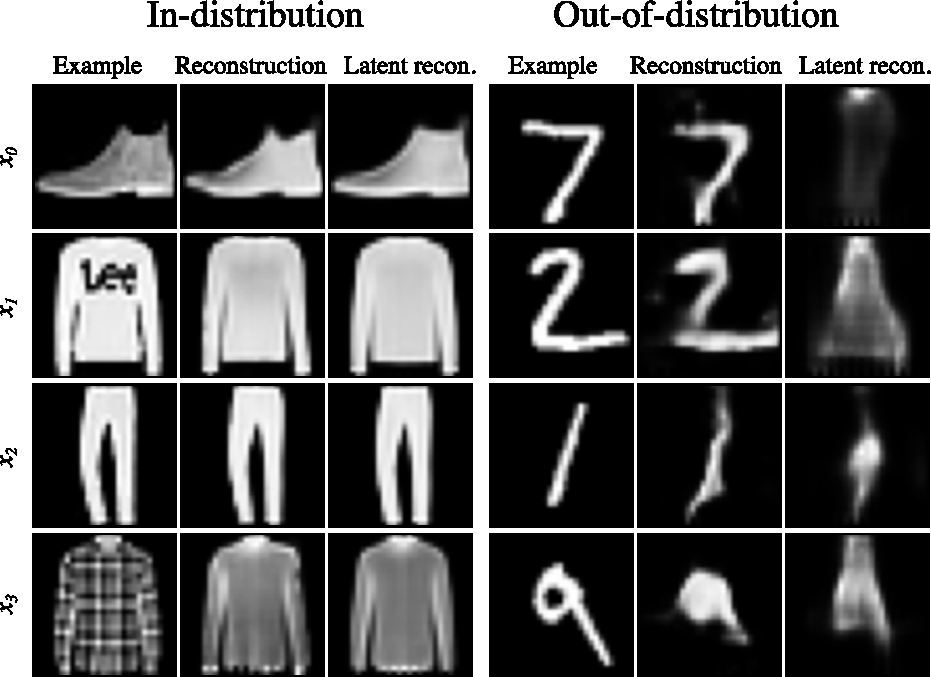
\includegraphics[height=\textheight]{../graphics/paper_hierarchical/reconstructions-front-page-4-samples-2-recons2.pdf}
    \end{figure}
\end{frame}


\begin{frame}
    \frametitle{Hierarchy of speech features}
    \begin{figure}
        \centering
        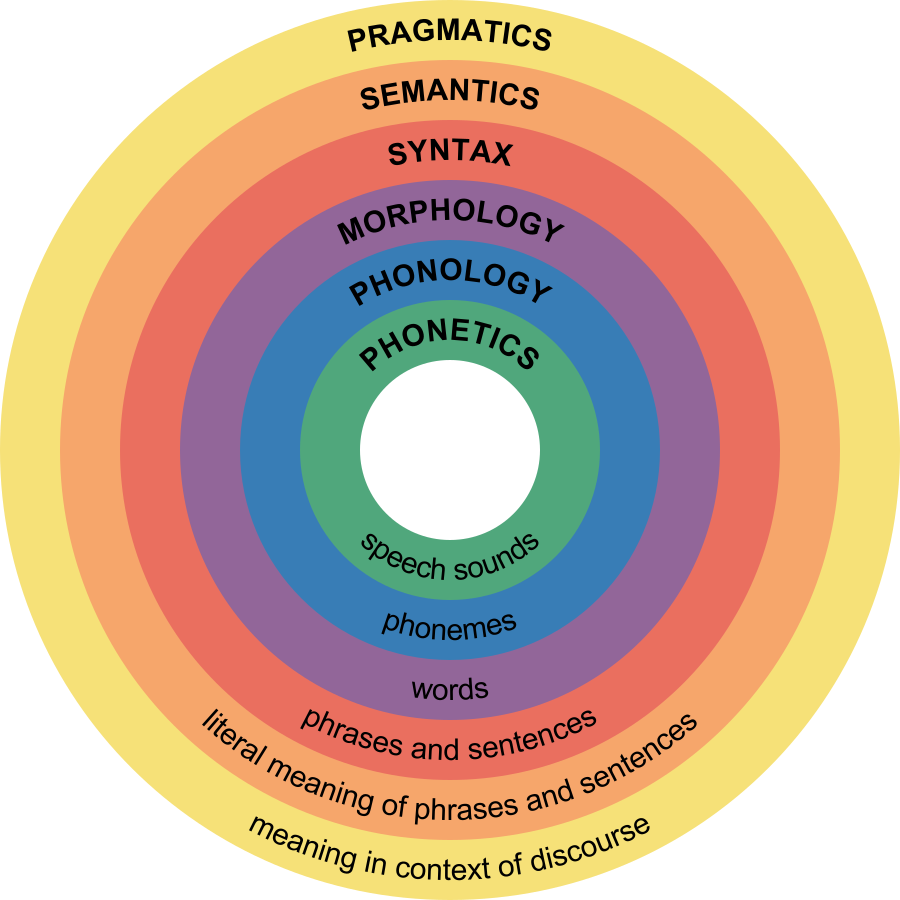
\includegraphics[height=\textheight]{figures/Major_levels_of_linguistic_structure.png}
    \end{figure}
\end{frame}


\begin{frame}
    \frametitle{Results on diverse datasets}
    \begin{columns}
        \begin{column}{0.45\textwidth}
            \hfill
            \begin{table}[t]
                \centering
                \resizebox{0.9\textwidth}{!}{%
                \begin{tabular}{llrrr}
                    \toprule
                    OOD dataset & Metric & AUROC$\uparrow$ & AUPRC$\uparrow$ & FPR80$\downarrow$ \\
                    \midrule
                    \multicolumn{5}{c}{\textbf{Trained on CIFAR10}} \\
                    \midrule
                    SVHN          &  $LLR^{>2}$  &  0.811  &  0.837  &  0.394  \\
                    CIFAR10       &  $LLR^{>1}$  &  0.469  &  0.479  &  0.835  \\
                    \midrule
                    \multicolumn{5}{c}{\textbf{Trained on SVHN}} \\
                    \midrule
                    CIFAR10            &  $LLR^{>1}$       &  $0.939$  &  $0.950$  &  $0.052$  \\
                    SVHN               &  $LLR^{>1}$       &  $0.489$  &  $0.484$  &  $0.799$  \\
                    \bottomrule
                \end{tabular}
                }
            \end{table}
            \hfill
        \end{column}
        \begin{column}{0.55\textwidth}
            \hfill
            \begin{table}[t]
                \centering
                \resizebox{0.9\textwidth}{!}{%
                \begin{tabular}{llrrr}
                    \toprule
                    OOD dataset & Metric & AUROC$\uparrow$ & AUPRC$\uparrow$ & FPR80$\downarrow$ \\
                    \midrule
                    \multicolumn{5}{c}{\textbf{Trained on FashionMNIST}} \\
                    \midrule
                    MNIST                    & $LLR^{>1}$             &  0.986  &  0.987  &  0.011 \\
                    notMNIST                 &  $LLR^{>1}$            &  0.998  &  0.998  &  0.000 \\
                    KMNIST                   &  $LLR^{>1}$            &  0.974  &  0.977  &  0.017 \\
                    Omniglot28x28            &  $LLR^{>2}$            &  1.000  &  1.000  &  0.000 \\
                    Omniglot28x28Inverted    &  $LLR^{>1}$            &  0.954  &  0.954  &  0.050 \\
                    SmallNORB28x28           &  $LLR^{>2}$            &  0.999  &  0.999  &  0.002 \\
                    SmallNORB28x28Inverted   &  $LLR^{>2}$            &  0.941  &  0.946  &  0.069 \\
    {\color{black!60}FashionMNIST}             &  $LLR^{>1}$            &  0.488  &  0.496  &  0.811 \\
                    \midrule
                    \multicolumn{5}{c}{\textbf{Trained on MNIST}} \\
                    \midrule
                    FashionMNIST                   &  $LLR^{>1}$  &  $0.999$  &  $0.999$  &  $0.000$ \\
                    notMNIST                       &  $LLR^{>1}$  &  $1.000$  &  $0.999$  &  $0.000$ \\
                    KMNIST                         &  $LLR^{>1}$  &  $0.999$  &  $0.999$  &  $0.000$ \\
                    Omniglot28x28                  &  $LLR^{>1}$  &  $1.000$  &  $1.000$  &  $0.000$ \\
                    Omniglot28x28Inverted          &  $LLR^{>1}$  &  $0.944$  &  $0.953$  &  $0.057$ \\
                    SmallNORB28x28                 &  $LLR^{>1}$  &  $1.000$  &  $1.000$  &  $0.000$ \\
                    SmallNORB28x28Inverted         &  $LLR^{>1}$  &  $0.985$  &  $0.987$  &  $0.000$ \\
    {\color{black!60}MNIST}                          &  $LLR^{>2}$  &  $0.515$  &  $0.507$  &  $0.792$ \\
                    \bottomrule
                \end{tabular}
                }
            \end{table}
            \hfill
        \end{column}
    \end{columns}
\end{frame}


% ======================================================================================================================


\section[A Brief Overview of Unsupervised Speech Representation Learning]{a brief overview of unsupervised speech representation learning}\label{extra:brief}


\begin{frame}
    \frametitle{Types of self-supervised speech representation learning methods}
    
    Schematic of self-supervised methods. Each subfigure illustrates the loss computation for a single time-step. The temporal subscript has been left out for simplicity.

    \begin{figure}
        \centering
        \setlength\tabcolsep{1.5pt}
        \resizebox*{\textheight}{!}{%
        \begin{tabular}{>{\centering\arraybackslash} m{4mm}  >{\centering\arraybackslash} m{0.40\textwidth}|>{\centering\arraybackslash} m{0.40\textwidth}}
            & {\small \textsc{predictive}} & {\small \textsc{masking-based}} \\
            \rotatebox{90}{{\small \textsc{reconstruct}}} & 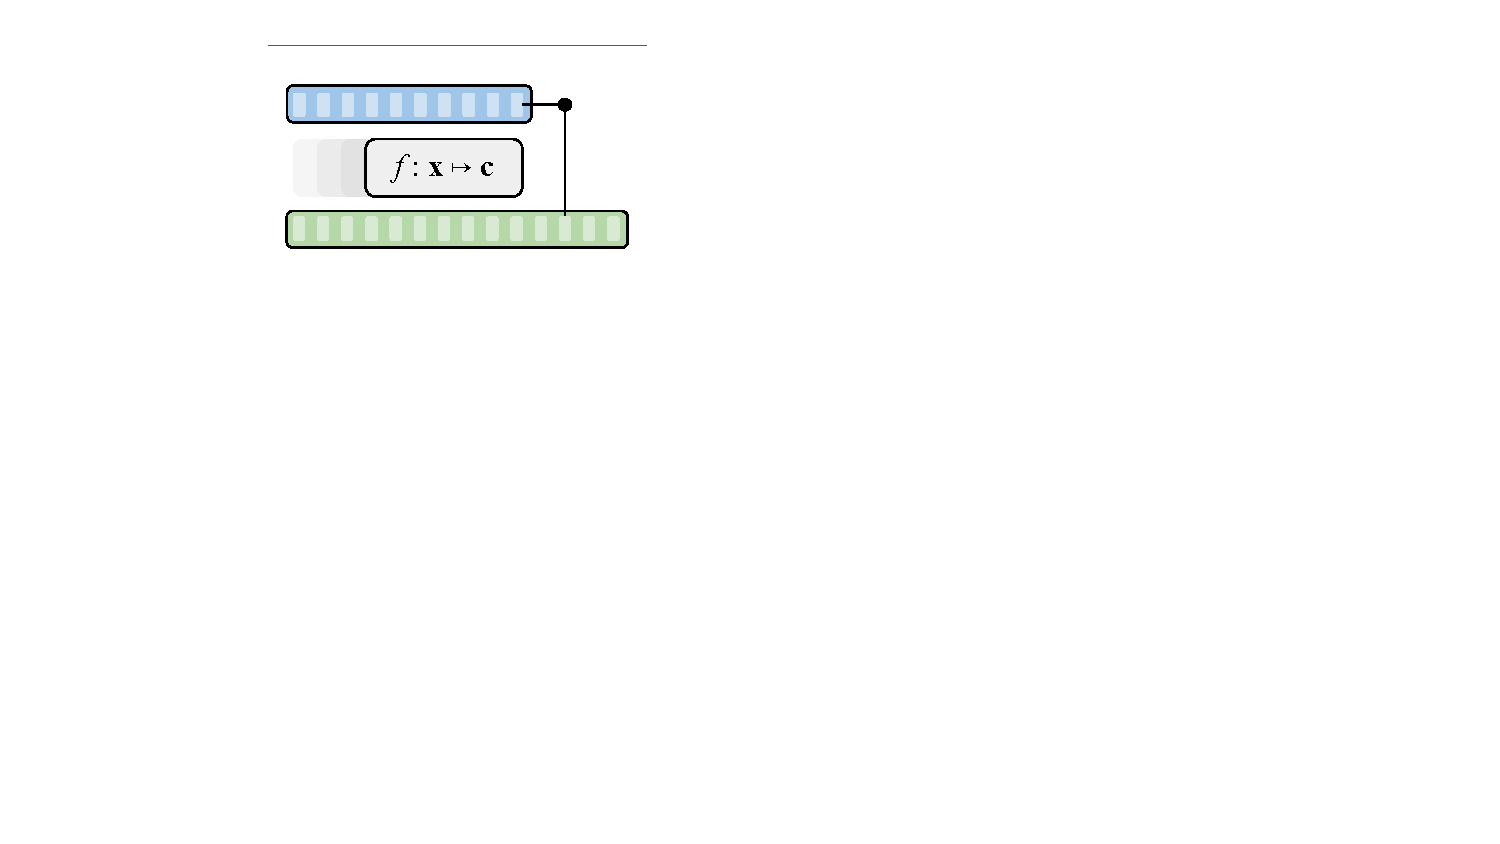
\includegraphics[width=0.40\textwidth]{../graphics/paper_brief/REC_PRD.pdf} & 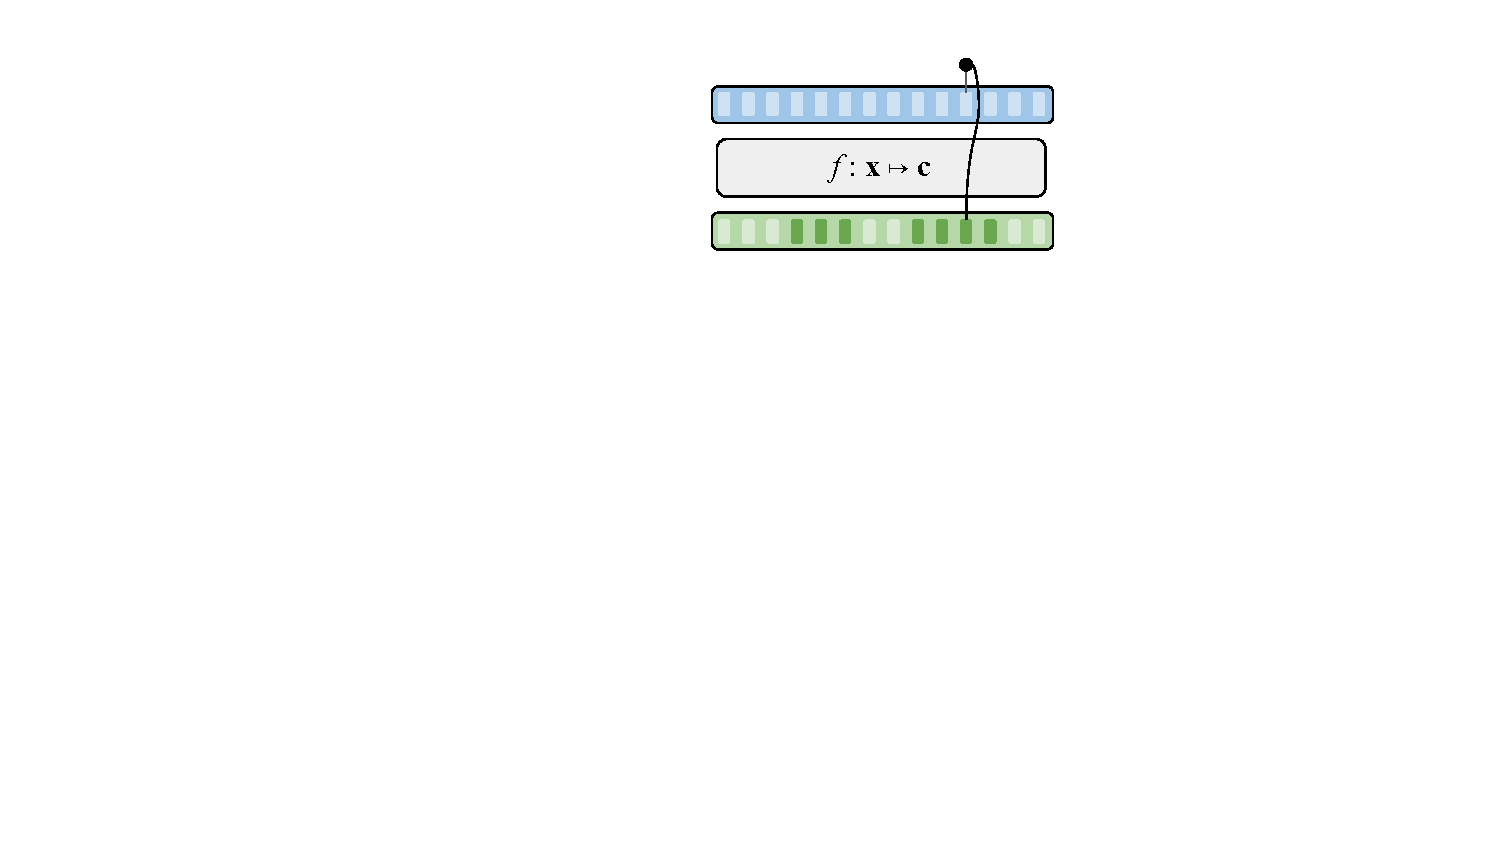
\includegraphics[width=0.40\textwidth]{../graphics/paper_brief/REC_MSK.pdf}  \\
            \midrule
            \rotatebox{90}{{\small \textsc{contrastive}}} & 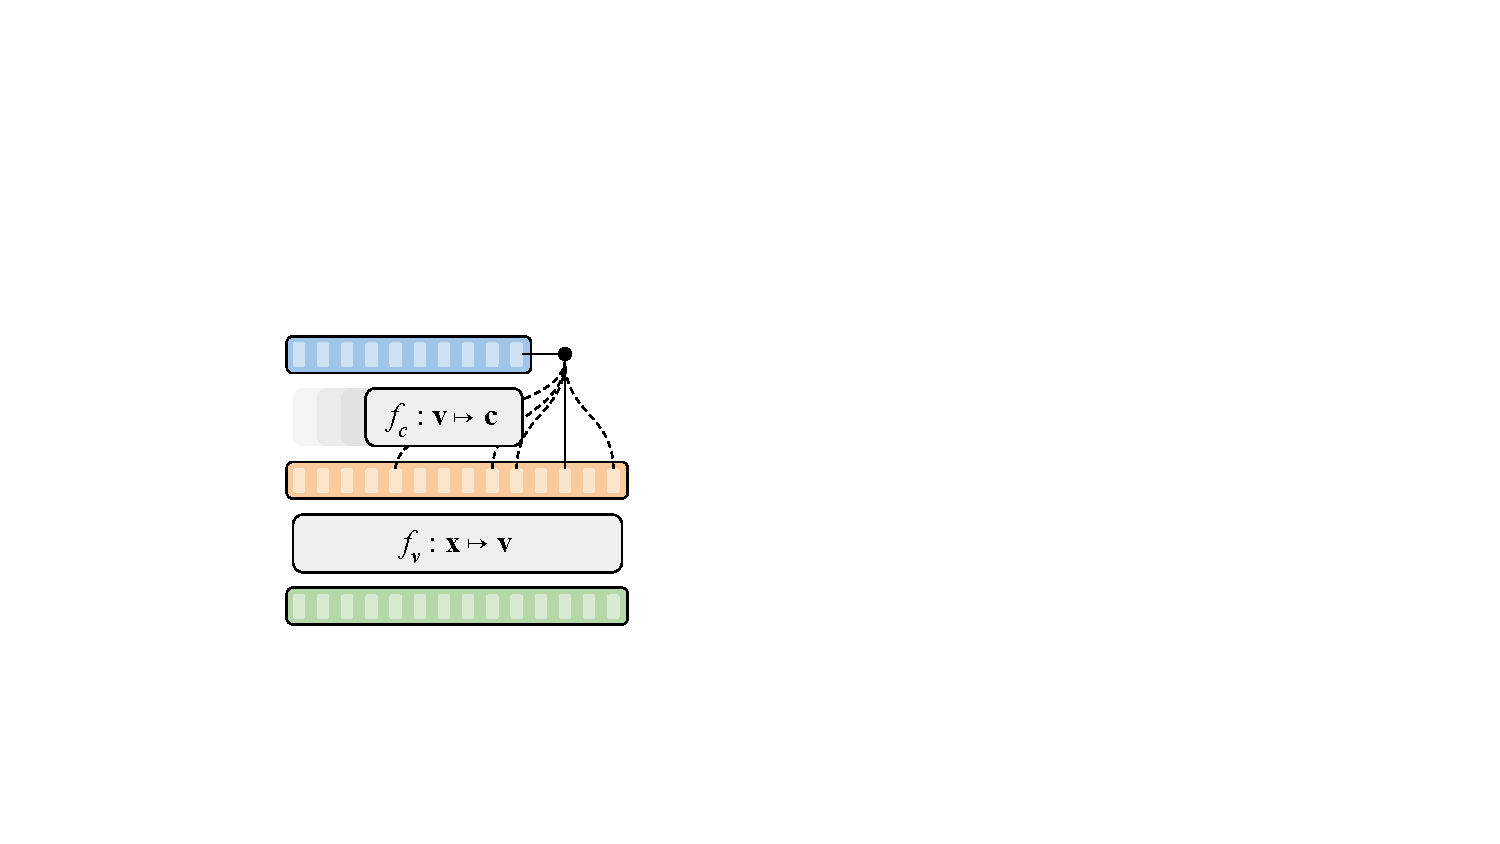
\includegraphics[width=0.40\textwidth]{../graphics/paper_brief/CON_PRD.pdf} & 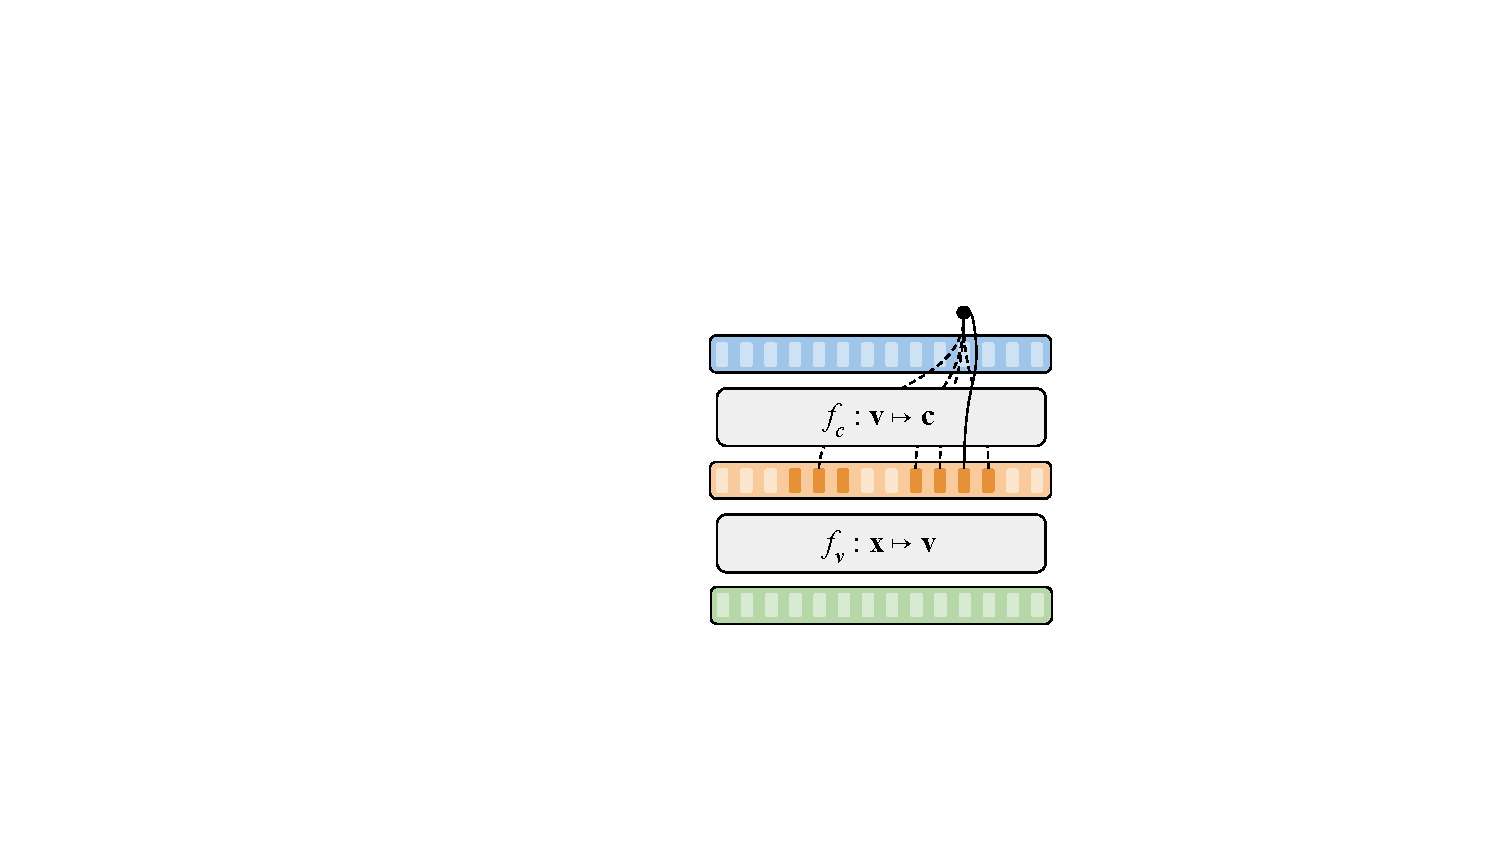
\includegraphics[width=0.40\textwidth]{../graphics/paper_brief/CON_MSK.pdf}
        \end{tabular}
        }
    \end{figure}
\end{frame}


\begin{frame}
    \frametitle{Overview: Representation Learning for Speech}

    \begin{columns}

        \begin{column}{0.4\textwidth}
            \begin{itemize}
                \item We focus on two primary categories:
                \begin{itemize}
                    \item Self-supervised learning (SSL)
                    \item Probabilistic latent variable models (LVMs)
                \end{itemize}
                \item Recent developments have been driven by self-supervised learning.
                \item A model-by-model overview: Focus on speech recognition.
            \end{itemize}
        \end{column}

        \begin{column}{0.6\textwidth}

            \begin{tikzpicture}
                \only<1->{
                    \node[anchor=south west,inner sep=0] (A) at (0,0) {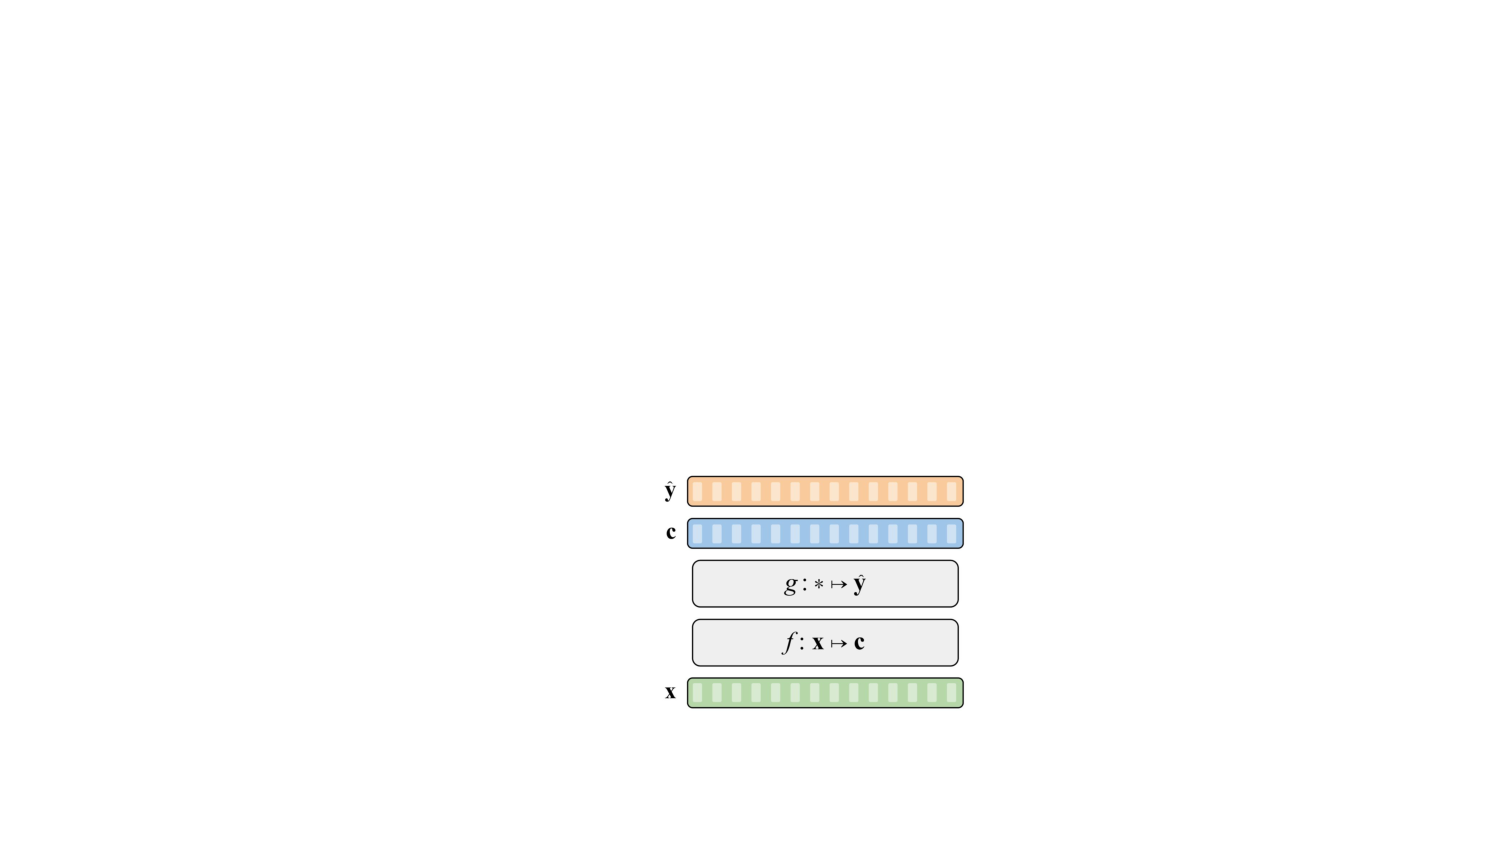
\includegraphics[height=0.4\textheight]{figures/brief-paradigms-ssl.pdf}};
                    \node[anchor=south west,inner sep=0] (B) at (4.2,0) {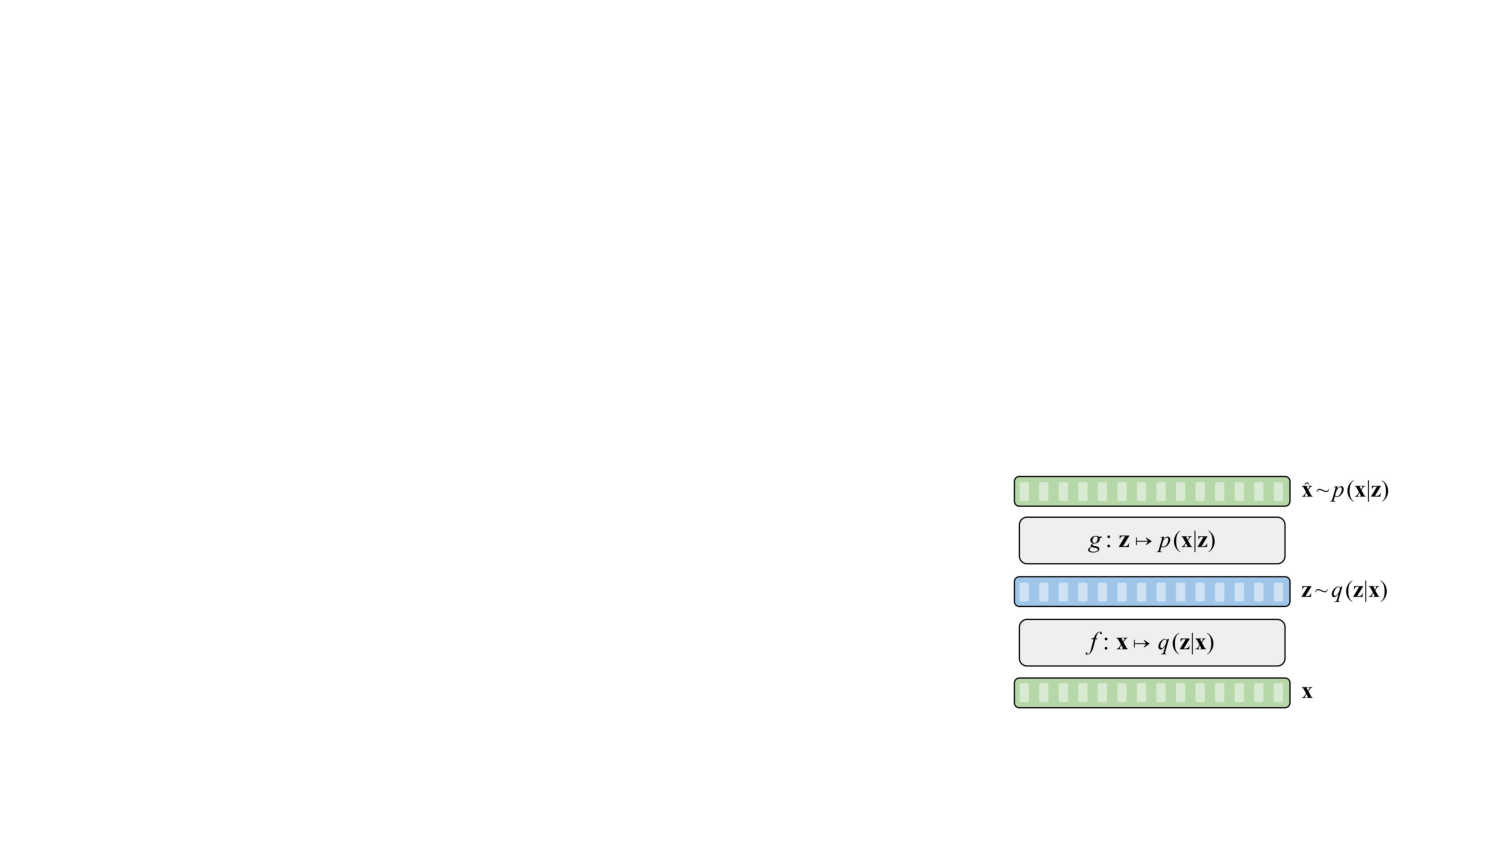
\includegraphics[height=0.4\textheight]{figures/brief-paradigms-lvm-2.pdf}};
                    \fill [draw=none, fill=white, fill opacity=0.7] (B.north west) -- (B.north east) -- (B.south east) -- (B.south west) -- (B.north west) -- cycle;
                }

                \only<2->{
                    \node[anchor=south west,inner sep=0] (A) at (0,0) {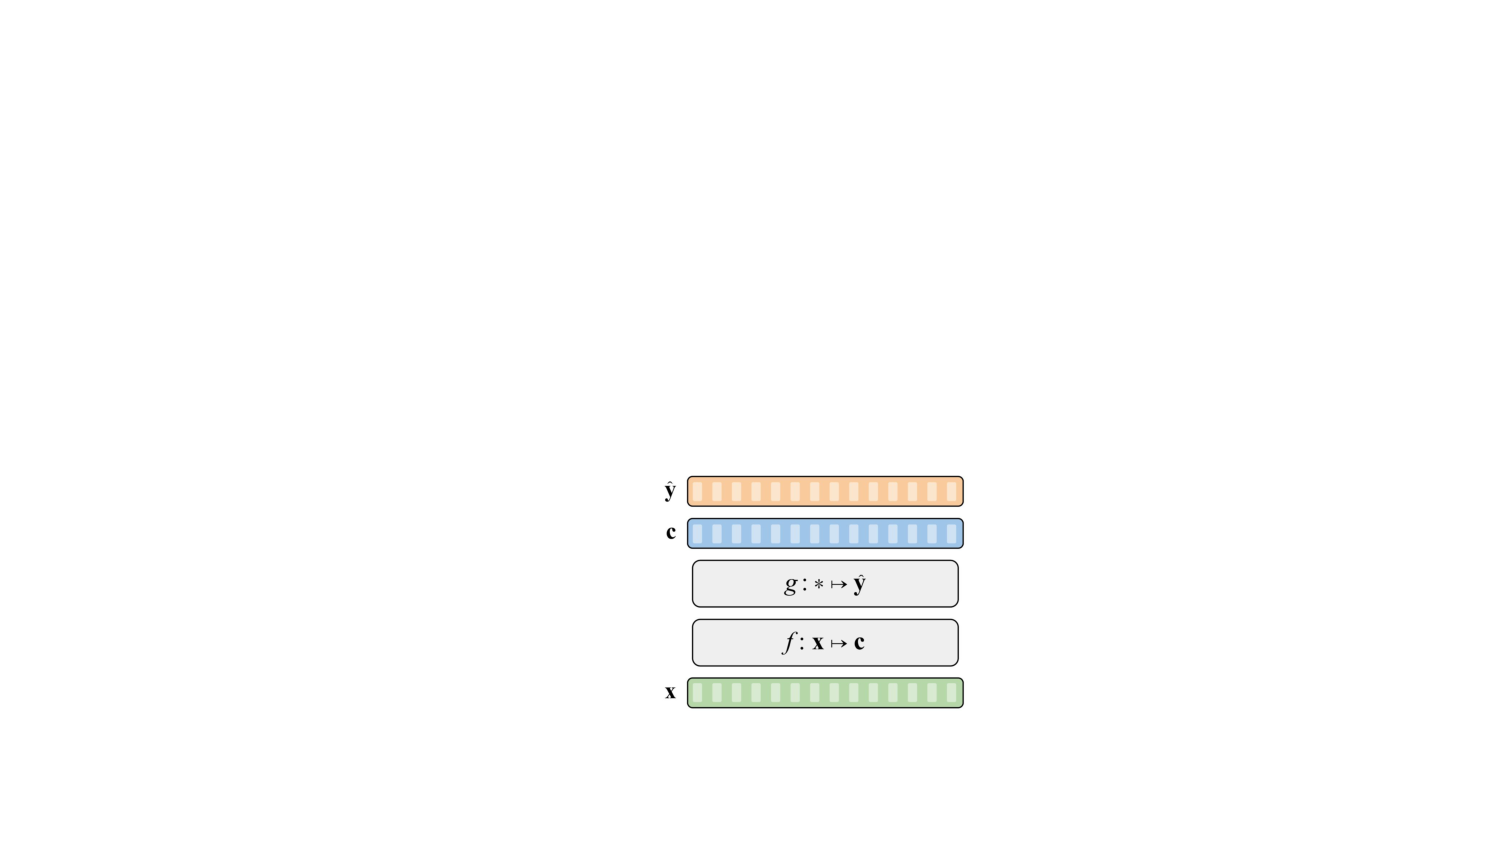
\includegraphics[height=0.4\textheight]{figures/brief-paradigms-ssl.pdf}};
                    \node[anchor=south west,inner sep=0] (B) at (4.2,0) {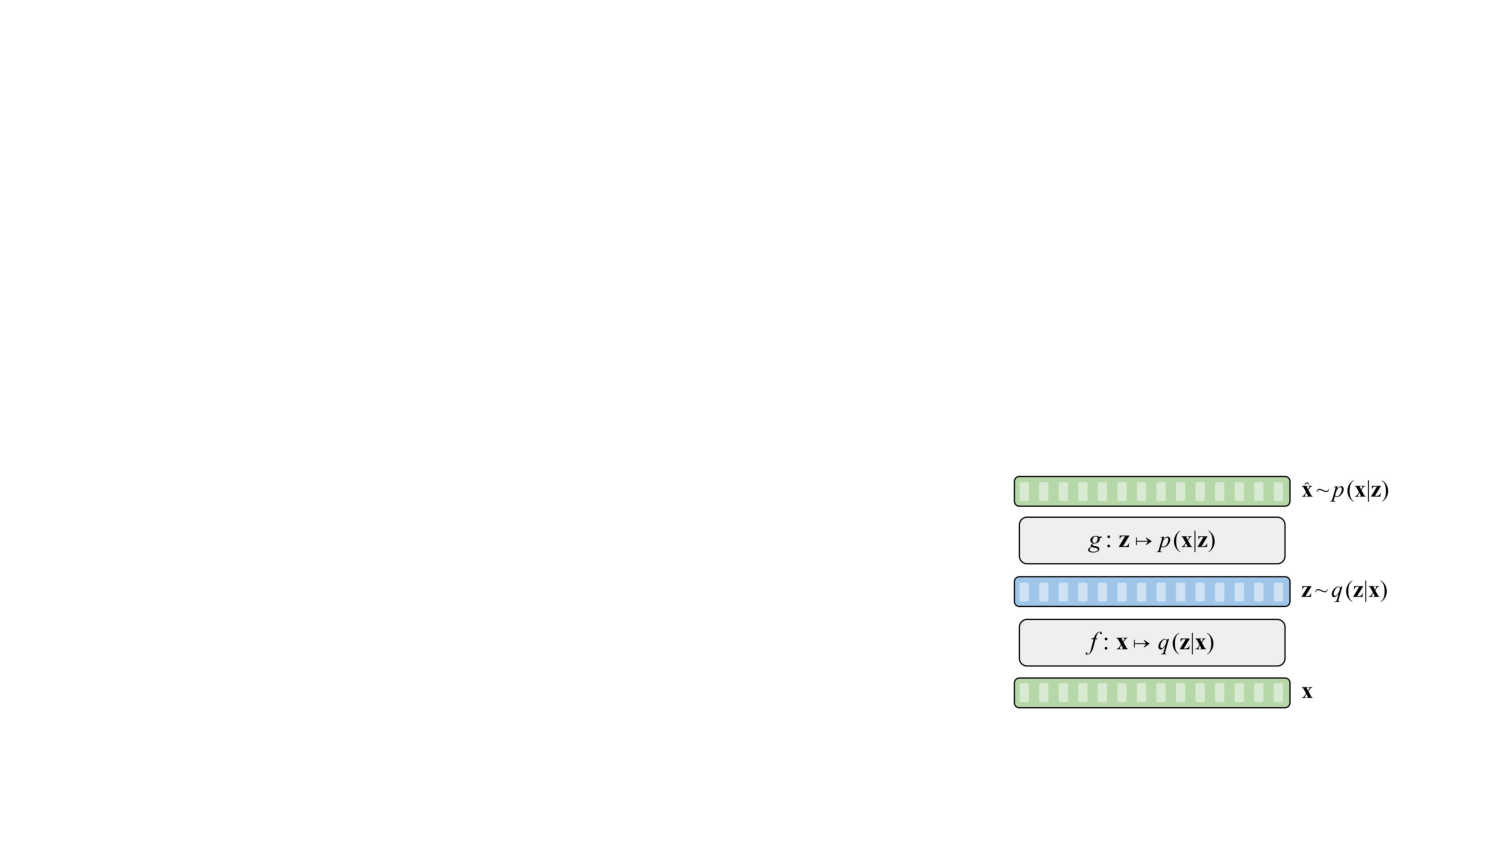
\includegraphics[height=0.4\textheight]{figures/brief-paradigms-lvm-2.pdf}};
                    \fill [draw=none, fill=white, fill opacity=0.7] (A.north west) -- (A.north east) -- (A.south east) -- (A.south west) -- (A.north west) -- cycle;
                }
            \end{tikzpicture}

        \end{column}
        
    \end{columns}
\end{frame}


\begin{frame}
    \frametitle{Graphical models for LVMs}
    % Figure TikZ sources at https://www.overleaf.com/project/61b212df9f315b5aec2b4a33
    \begin{columns}

        \begin{column}{0.5\textwidth}
            \begin{figure}
                \centering
                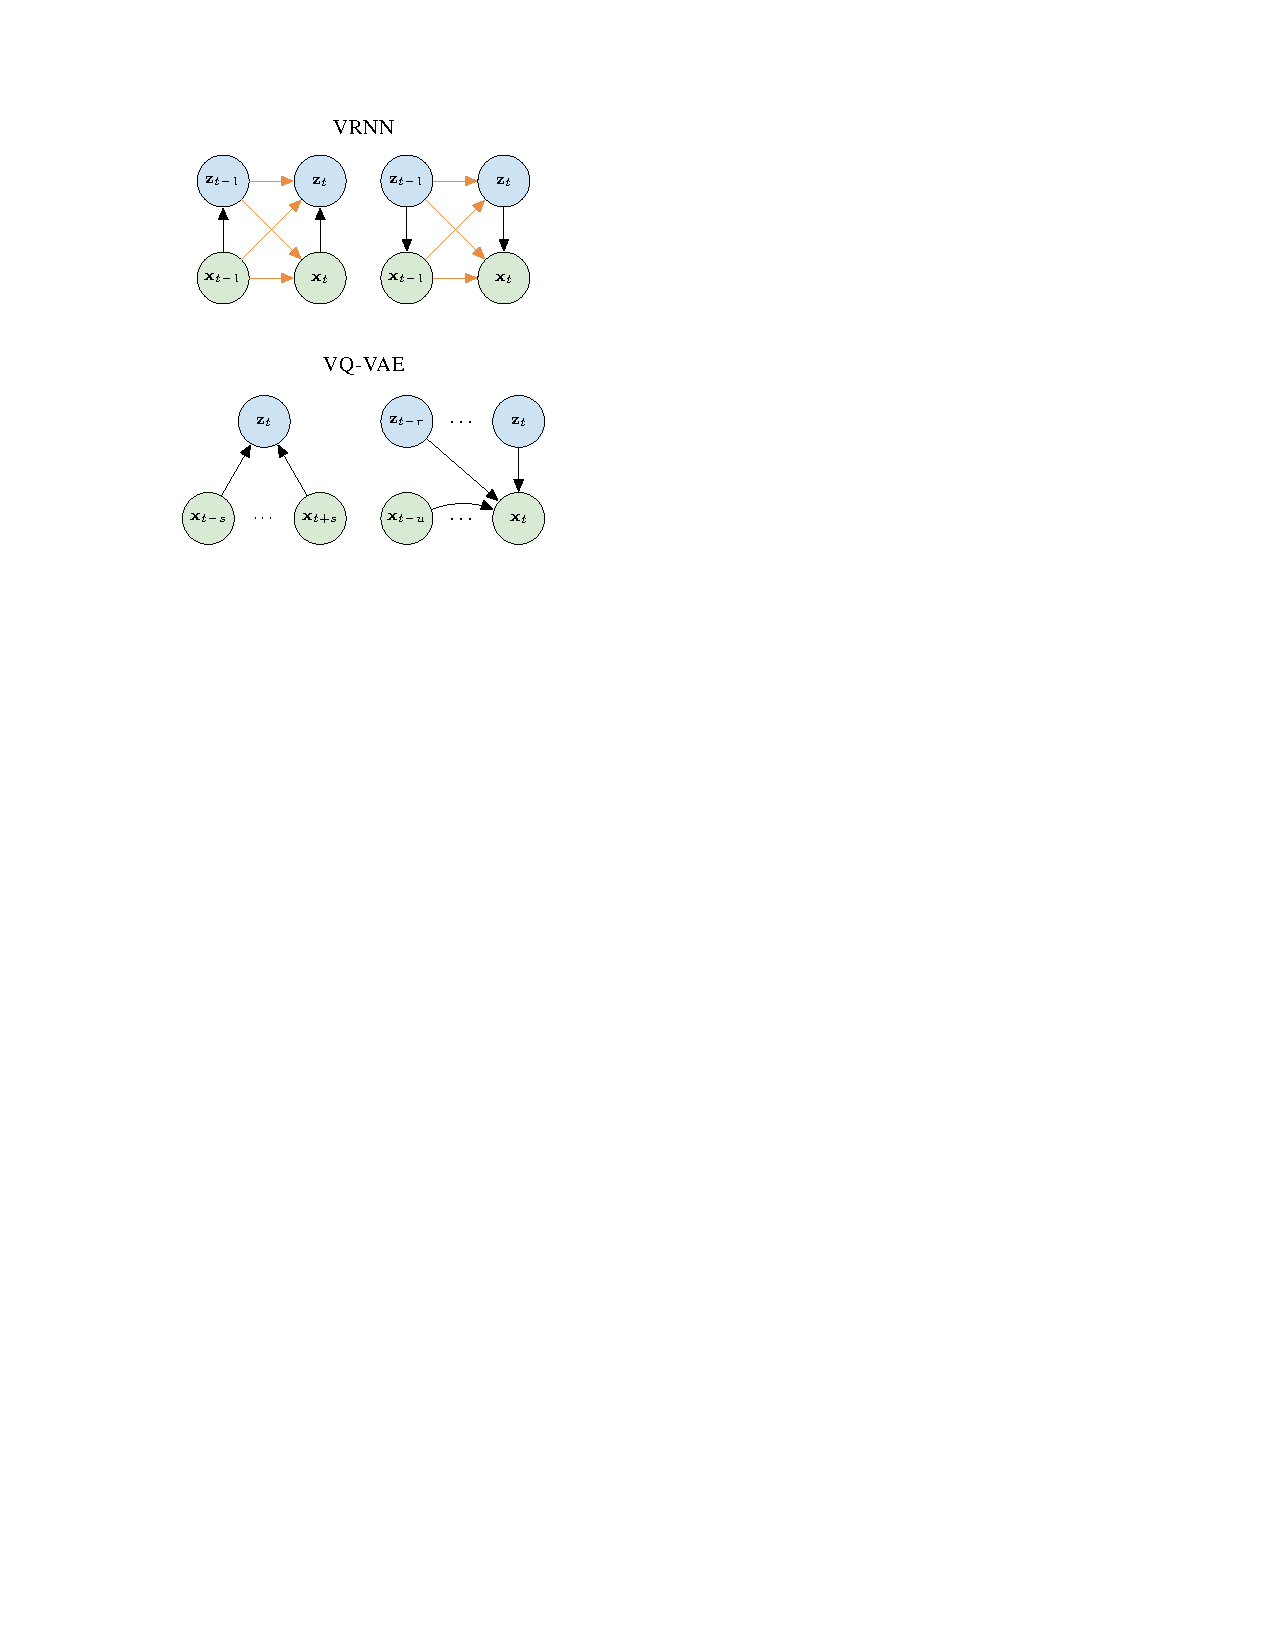
\includegraphics[width=0.8\textwidth]{figures/brief-vrnn-vqvae.pdf}
            \end{figure}
        \end{column}

        \begin{column}{0.5\textwidth}
            \begin{figure}
                \centering
                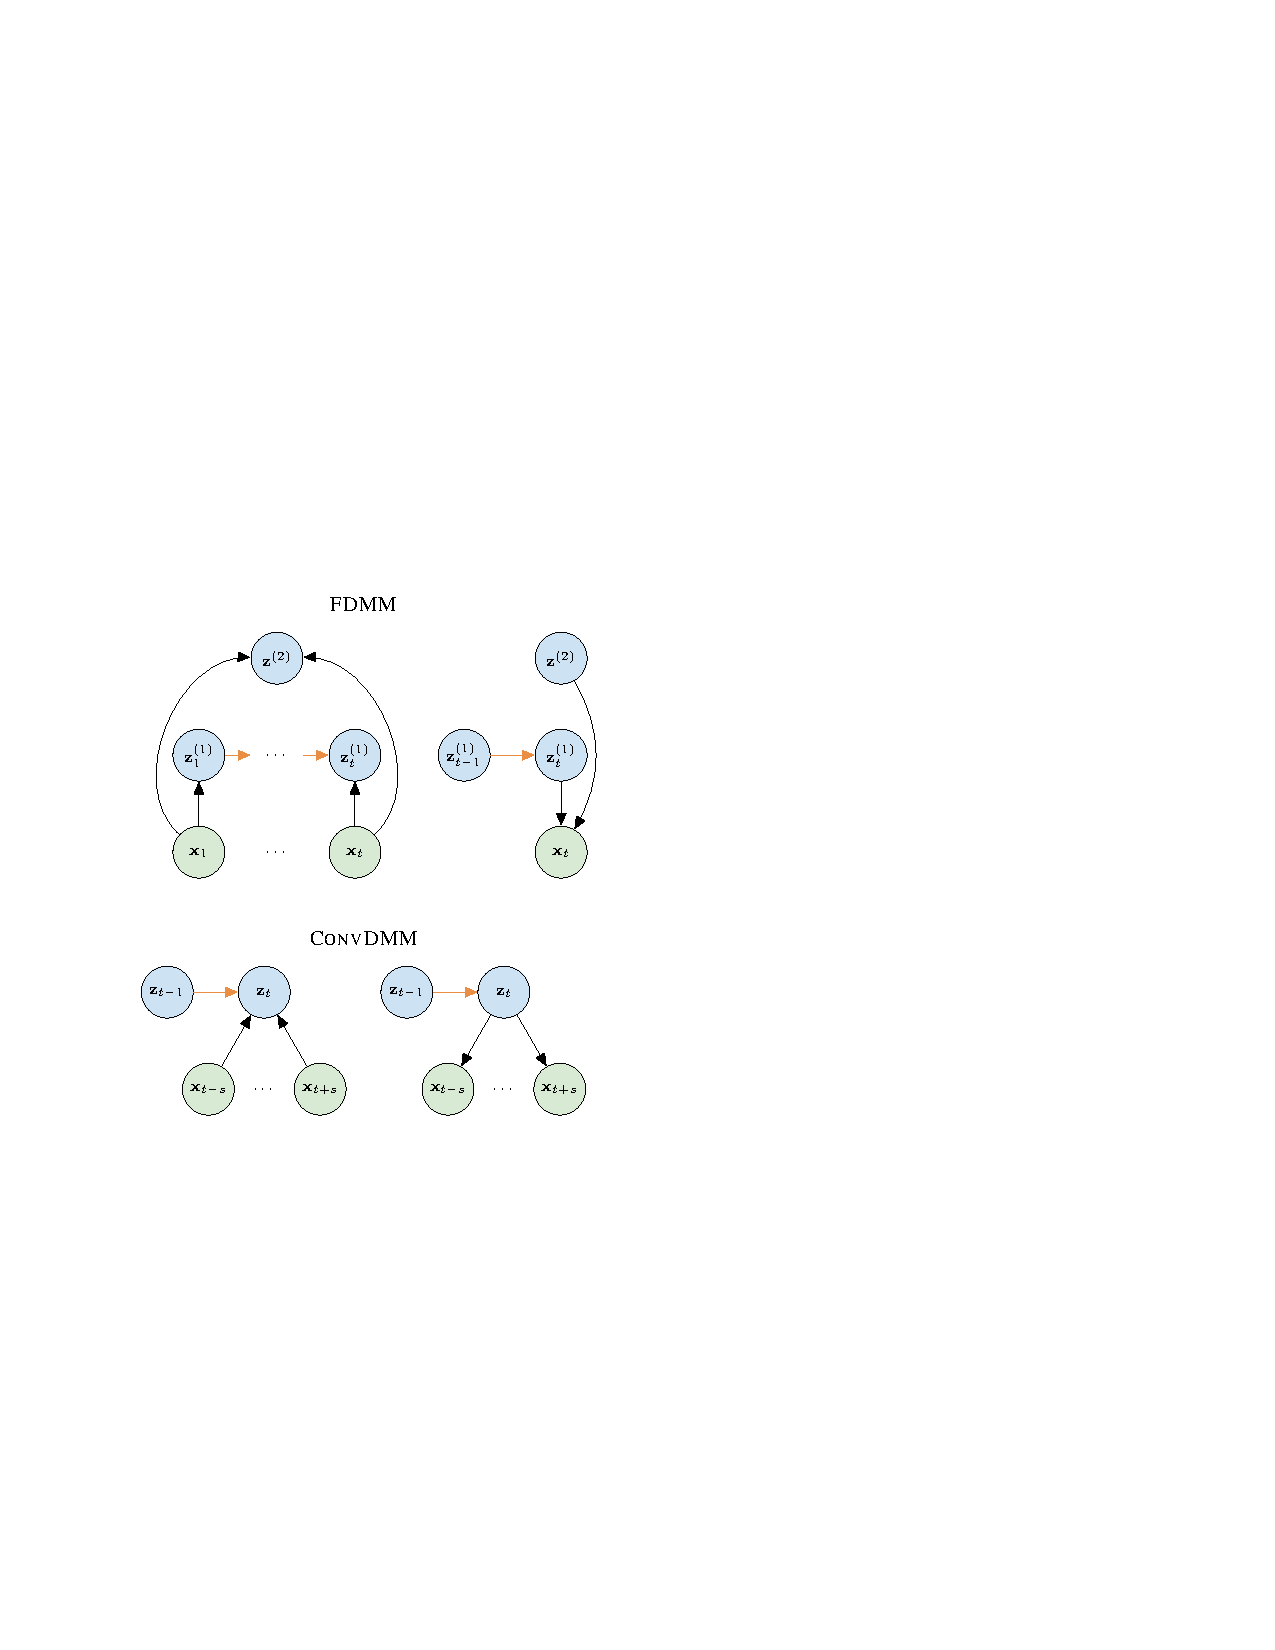
\includegraphics[width=0.8\textwidth]{figures/brief-fdmm-convdmm.pdf}
            \end{figure}            
        \end{column}

    \end{columns}

    \definecolor{sharedcolor}{RGB}{234 142 67} % mørk orange
    \blfootnote{\scalebox{0.6}{{\color{sharedcolor} Orange edges} indicate parameters shared between inference and generative models.}}
\end{frame}


\begin{frame}
    \frametitle{Overview of LVM probabilistic components}

    \begin{table}
        \centering
        \resizebox{0.8\textheight}{!}{%
            \begin{tabular}{ l l l } 
                \toprule
                \multicolumn{2}{l}{\textbf{\textsc{Type}}} & \textbf{\textsc{Form}} \\
                \midrule
                \multicolumn{3}{c}{\textsc{Observation model}} \\
                \midrule
                \textbf{\textsc{arx}} & Autoregressive on $\mathbf{x}_t$      & $p(\mathbf{x}_t|\mathbf{x}_{1:t-1})$ \\
                \textbf{\textsc{loc}} & Local latent variable                 & $p(\mathbf{x}_{t}|\mathbf{z}_{1:t})$ \\
                \textbf{\textsc{glb}} & Global latent variable                & $p(\mathbf{x}_{t}|\mathbf{z})$ \\
                \midrule
                \multicolumn{3}{c}{\textsc{Prior}} \\
                \midrule
                \textbf{\textsc{arx}} & Autoregressive on $\mathbf{x}_t$      & $p(\mathbf{z}_t|\mathbf{x}_{1:t-1})$ \\
                \textbf{\textsc{arz}} & Autoregressive on $\mathbf{z}_t$      & $p(\mathbf{z}_t|\mathbf{z}_{1:t-1})$ \\
                \textbf{\textsc{ind}} & Locally independent $\mathbf{z}_t$                 & $p(\mathbf{z}_t)$ \\
                \textbf{\textsc{glb}} & Global latent variable                & $p(\mathbf{z})$ \\
                \midrule
                \multicolumn{3}{c}{\textsc{Inference model}} \\
                \midrule
                \textbf{\textsc{arz}} & Autoregressive on $\mathbf{z}_t$      & $q(\mathbf{z}_t|\mathbf{z}_{1:t-1})$ \\
                \textbf{\textsc{flt}} & Filtering                             & $q(\mathbf{z}_t|\mathbf{x}_{1:t})$ \\
                \textbf{\textsc{lsm}} & Local smoothing                       & $q(\mathbf{z}_t|\mathbf{x}_{t-r:t+r})$ \\
                \textbf{\textsc{gsm}} & Global smoothing                      & $q(\mathbf{z}_t|\mathbf{x}_{1:T})$ \\
                \textbf{\textsc{glb}} & Global latent variable                & $q(\mathbf{z}|\mathbf{x}_{1:T})$ \\
                \bottomrule
            \end{tabular}
        }
    \end{table}

\end{frame}


\begin{frame}
    \frametitle{Classification of selected LVMs for speech}

    \begin{table}
        \centering
        \setlength{\tabcolsep}{3pt}
        \renewcommand{\arraystretch}{1.1}
        \resizebox{0.7\textwidth}{!}{%
            \begin{tabular}{ l | c c c | c c c c | c c c c c | c } 
                \toprule
                \multicolumn{2}{c}{} & 
                \multicolumn{3}{c}{\textsc{Observation}} & 
                \multicolumn{4}{c}{\textsc{Prior}} & 
                \multicolumn{5}{c}{\textsc{Inference}} \\
                \textbf{\textsc{model}} & 
                \textbf{\textsc{arx}} & 
                \textbf{\textsc{loc}} & 
                \textbf{\textsc{glb}} &  
                \textbf{\textsc{arx}} & 
                \textbf{\textsc{arz}} & 
                \textbf{\textsc{ind}} & 
                \textbf{\textsc{glb}} &  
                \textbf{\textsc{arz}} & 
                \textbf{\textsc{flt}} & 
                \textbf{\textsc{lsm}} & 
                \textbf{\textsc{gsm}} & 
                \textbf{\textsc{glb}} &
                \textbf{\textsc{hie}} \\
                \midrule
                %                                                              OBSERVATION       |              PRIOR                |                  INFERENCE       
                %                                                         ARX      LOC      GLB      ARX      ARZ     IND      GLB      ARZ      FLT      LSM      GSM      GLB
                \textbf{VRNN} \footnotesize{\parencite{chung_recurrent_2015}}          & \cmark & \cmark & \xmark & \cmark & \cmark & \xmark & \xmark & \cmark & \cmark & \xmark & \xmark & \xmark & \xmark \\
                \textbf{SRNN} \footnotesize{\parencite{fraccaro_sequential_2016}}      & \cmark & \cmark & \xmark & \cmark & \cmark & \xmark & \xmark & \cmark & \xmark & \xmark & \cmark & \xmark & \xmark \\
                \textbf{HMM-VAE} \footnotesize{\parencite{ebbers_hidden_2017}}         & \xmark & \cmark & \xmark & \xmark & \cmark & \xmark & \xmark & \cmark & \cmark & \xmark & \xmark & \xmark & \cmark \\
                \textbf{ConvVAE} \footnotesize{\parencite{hsu_learning_2017}}          & \xmark & \xmark & \cmark & \xmark & \xmark & \xmark & \cmark & \xmark & \xmark & \xmark & \cmark & \cmark & \xmark \\
                \textbf{FHVAE} \footnotesize{\parencite{hsu_unsupervised_2017}}        & \xmark & \cmark & \cmark & \xmark & \xmark & \cmark & \cmark & \xmark & \xmark & \xmark & \cmark & \cmark & \cmark \\
                \textbf{VQ-VAE} \footnotesize{\parencite{oord_neural_2018}}            & \cmark & \cmark & \xmark & \xmark & \xmark & \cmark & \xmark & \xmark & \xmark & \cmark & \xmark & \xmark & \xmark \\
                \textbf{BHMM-VAE} \footnotesize{\parencite{glarner_full_2018}}         & \xmark & \cmark & \xmark & \xmark & \cmark & \xmark & \xmark & \cmark & \cmark & \xmark & \xmark & \xmark & \xmark \\
                \textbf{STCN} \footnotesize{\parencite{aksan_stcn_2019}}               & \xmark & \cmark & \xmark & \cmark & \xmark & \xmark & \xmark & \xmark & \cmark & \xmark & \xmark & \xmark & \cmark \\
                \textbf{FDMM} \footnotesize{\parencite{khurana_factorial_2019}}        & \xmark & \cmark & \cmark & \xmark & \cmark & \xmark & \cmark & \cmark & \cmark & \xmark & \xmark & \cmark & \cmark \\
                \textbf{ConvDMM} \footnotesize{\parencite{khurana_convolutional_2020}} & \xmark & \cmark & \xmark & \xmark & \cmark & \xmark & \xmark & \cmark & \xmark & \cmark & \xmark & \xmark & \xmark \\
                \bottomrule
            \end{tabular}
        }
    \end{table}

\end{frame}

\begin{frame}
    \frametitle{Comparison of LVMs and SSL methods}

    \begin{table}
        \centering
        \setlength{\tabcolsep}{3pt}
        \renewcommand{\arraystretch}{1.1}
        \resizebox{1\textheight}{!}{%
            \begin{tabular}{ l l | c c c c c c | c c c | c c } 
                \toprule
                
                \multicolumn{2}{c}{} & 
                \multicolumn{6}{c}{\textsc{model and task design}} & 
                \multicolumn{3}{c}{\textsc{resolution}} &
                \multicolumn{2}{c}{\makebox[0pt][c]{\textsc{usage}}} \\
                & \textbf{\textsc{model}} &
                \textbf{\textsc{msk}} & 
                \textbf{\textsc{prd}} & 
                \textbf{\textsc{con}} &  
                \textbf{\textsc{rec}} &  
                \textbf{\textsc{qtz}} & 
                \textbf{\textsc{gen}} & 
                \textbf{\textsc{loc}} & 
                \textbf{\textsc{glb}} & 
                \textbf{\textsc{var}} & 
                \textbf{\textsc{frz}} & 
                \textbf{\textsc{ftn}} \\
                
                \midrule
                % \multicolumn{11}{c}{\textsc{Self-supervised models}} \\
                % \midrule
                %                                                           MSK      PRD      CON      REC      QTZ      GEN      LOC      GLB     VAR      FRZ      FTN
                \verticalmultirow{9}{\textsc{Self-supervised models}} 
                % & \textbf{Audio Word2vec} \footnotesize{\parencite{chung_audio_2016}}      & \cmark & \xmark & \xmark & \cmark & \xmark & \xmark & \xmark & \cmark & \xmark & \cmark & \xmark \\
                % & \textbf{Speech2Vec} \footnotesize{\parencite{chung_speech2vec_2018}}     & \xmark & \cmark & \xmark & \cmark & \xmark & \xmark & \xmark & \cmark & \xmark & \cmark & \xmark \\
                % & \textbf{Unspeech} \footnotesize{\parencite{milde_unspeech_2018}}         & \xmark & \cmark & \cmark & \xmark & \xmark & \xmark & \xmark & \cmark & \xmark & \cmark & \xmark \\
                
                & \textbf{CPC} \footnotesize{\parencite{oord_representation_2018}}         & \xmark & \cmark & \cmark & \xmark & \xmark & \xmark & \cmark & \xmark & \xmark & \cmark & \xmark \\
                
                & \textbf{APC} \footnotesize{\parencite{chung_unsupervised_2019}}          & \xmark & \cmark & \xmark & \cmark & \xmark & \xmark & \cmark & \xmark & \xmark & \cmark & \xmark \\ % 5/4
                & \textbf{wav2vec} \footnotesize{\parencite{schneider_wav2vec_2019}}       & \xmark & \cmark & \cmark & \xmark & \xmark & \xmark & \cmark & \xmark & \xmark & \cmark & \xmark \\ % 11/4
                & \textbf{Mockingjay}  \footnotesize{\parencite{liu_mockingjay_2020}}      & \cmark & \xmark & \xmark & \cmark & \xmark & \xmark & \cmark & \xmark & \xmark & \cmark & \cmark \\ % 25/10-19
                & \textbf{wav2vec 2.0} \footnotesize{\parencite{baevski_wav2vec_2020}}     & \cmark & \xmark & \cmark & \xmark & \cmark & \xmark & \cmark & \xmark & \xmark & \xmark & \cmark \\ % 20/6
                & \textbf{NPC} \footnotesize{\parencite{liu_nonautoregressive_2020}}       & \cmark & \xmark & \xmark & \cmark & \cmark & \xmark & \cmark & \xmark & \xmark & \cmark & \xmark \\ % 1/11
                & \textbf{DeCoAR 2.0} \footnotesize{\parencite{ling_decoar_2020}}          & \cmark & \xmark & \xmark & \cmark & \cmark & \xmark & \cmark & \xmark & \xmark & \cmark & \xmark \\ % 11/12
                % & \textbf{SCPC} \footnotesize{\parencite{bhati_segmental_2021}}            & \xmark & \cmark & \cmark & \xmark & \xmark & \xmark & \cmark & \xmark & \cmark & \cmark & \xmark \\ % 3/6
                & \textbf{HuBERT} \footnotesize{\parencite{hsu_hubert_2021}}               & \cmark & \xmark & \xmark & \xmark & \cmark & \xmark & \cmark & \xmark & \xmark & \xmark & \cmark \\ % 14/6
                & \textbf{data2vec} \footnotesize{\parencite{baevski_data2vec_2022}}       & \cmark & \xmark & \xmark & \xmark & \xmark & \xmark & \cmark & \xmark & \xmark & \xmark & \cmark \\ % 16/6

                \midrule
                % \multicolumn{11}{c}{\textsc{Probabilistic latent variable models}} \\
                % \midrule
                %                                                           MSK      PRD      CON      REC      QTZ      GEN      LOC      GLO     VAR      FRZ      FTN
                \verticalmultirow{8}{\textsc{Latent variable models}}
                & \textbf{VRNN} \footnotesize{\parencite{chung_recurrent_2015}}          & \xmark & \xmark & \xmark & \cmark & \xmark & \cmark & \cmark & \xmark & \xmark & \cmark & \xmark \\
                & \textbf{SRNN} \footnotesize{\parencite{fraccaro_sequential_2016}}      &\xmark & \xmark & \xmark & \cmark & \xmark & \cmark & \cmark & \xmark & \xmark & \cmark & \xmark \\
                % & \textbf{HMM-VAE} \footnotesize{\parencite{ebbers_hidden_2017}}         & \xmark & \xmark & \xmark & \cmark & \xmark & \cmark & \cmark & \xmark & \xmark & \cmark & \xmark \\
                & \textbf{ConvVAE} \footnotesize{\parencite{hsu_learning_2017}}          & \xmark & \xmark & \xmark & \cmark & \xmark & \cmark & \xmark & \cmark & \xmark & \cmark & \xmark \\
                & \textbf{FHVAE} \footnotesize{\parencite{hsu_unsupervised_2017}}        & \xmark & \xmark & \xmark & \cmark & \xmark & \cmark & \cmark & \cmark & \xmark & \cmark & \xmark \\
                & \textbf{VQ-VAE} \footnotesize{\parencite{oord_neural_2018}}            & \xmark & \xmark & \xmark & \cmark & \cmark & \cmark & \cmark & \xmark & \xmark & \cmark & \xmark \\
                % & \textbf{BHMM-VAE} \footnotesize{\parencite{glarner_full_2018}}         & \xmark & \xmark & \xmark & \cmark & \xmark & \cmark & \cmark & \xmark & \xmark & \cmark & \xmark \\
                & \textbf{STCN} \footnotesize{\parencite{aksan_stcn_2019}}               & \xmark & \xmark & \xmark & \cmark & \xmark & \cmark & \cmark & \xmark & \xmark & \cmark & \xmark \\
                & \textbf{FDMM} \footnotesize{\parencite{khurana_factorial_2019}}        & \xmark & \xmark & \xmark & \cmark & \xmark & \cmark & \cmark & \cmark & \xmark & \cmark & \xmark \\
                & \textbf{ConvDMM} \footnotesize{\parencite{khurana_convolutional_2020}} & \xmark & \xmark & \xmark & \cmark & \xmark & \cmark & \cmark & \xmark & \xmark & \cmark & \xmark \\
                \bottomrule
            \end{tabular}
        }
    \end{table}

\end{frame}


% ======================================================================================================================


\section[A Retrospective Study on Machine Learning-Assisted Stroke Recognition for Medical Helpline Calls]{a retrospective study on machine learning-assisted stroke recognition for medical helpline calls}\label{extra:retrospective}


\begin{frame}
    \frametitle{Simulated prospective study}
    \begin{enumerate}
        \item[I.] \highlight{When} is the model prediction presented to the call-taker?
        \begin{enumerate}
            \item[1.] Notify the call-taker \highlight{after the call ends}.
            \item[2.] Notify the call-taker \highlight{during the call}.
        \end{enumerate}
        \item[II.] \highlight{How} does prediction influence the diagnostic code the call-taker assigns to the call?
        \begin{enumerate}[label=\Alph*.]
            \item[A.] Call-takers \highlight{mirror model positives}.
            \item[B.] Call-takers \highlight{mirror model negatives}.
            \item[C.] Call-takers mirror model predictions (corresponds to main results of the model itself).
        \end{enumerate}
    \end{enumerate}
    \vspace{0.5em}
    To simulate the online scenario (2.), we \highlight{stream the transcript} to the model and make predictions every 50 words. 
    A stroke positive is triggered only when three consecutive positive predictions are made. 
    This is similar to the strategy implemented for a previous RCT on cardiac arrest \cite{cite15}.

        % %
        % Option 1 is identical to the method used in the main study. In option 2, predictions are made during the call based only on partial transcriptions. We implemented option 2 in such a manner that the model predicted every time 50 new words were transcribed and added to the transcript. A stroke positive was triggered only when three consecutive positive predictions were made (i.e., without intermediate negative stroke predictions). In other words, the sigmoid activation of the model had to remain above 0.5 for three consecutive predictions, for example, after 150, 200, and 250 words were transcribed.
        
        % As we can only assume how call takers are influenced by model predictions (II), precisely evaluating the hypothetical performance of call takers when supported by a machine learning framework is impossible. Furthermore, option 2 may influence the conversation, further complicating matters. Therefore, we report the results combining the call taker and the model under the following two assumptions:
        % %
\end{frame}


\begin{frame}
    \frametitle{Simulated prospective study}

    \begin{table}
        \centering
        \resizebox*{0.98\textwidth}{!}{%
        \begin{tabular}{l|c|cc|cc|cc}
            \toprule
    
            \textbf{Predictor} & \textbf{Call-taker} & \multicolumn{2}{c|}{\textbf{Model}} & \multicolumn{4}{c}{\textbf{Call-taker supported by the model (simulated)}} \\
            \midrule
            \textbf{When} & \textbf{During call} & \textbf{After call} & \textbf{During call} & \textbf{After call} & \textbf{During call} & \textbf{After call} & \textbf{During call} \\
            \midrule
            \textbf{Method} & - & - & - & \textbf{neg $\rightarrow$ pos} & \textbf{neg $\rightarrow$ pos} & \textbf{pos $\rightarrow$ neg} & \textbf{pos $\rightarrow$ neg} \\
            \midrule
    
            \makecell[l]{\textbf{F1-score} [\%] $\uparrow$}                             & \makecell[c]{25.8 \\ \shade{(23.7-27.9)}} & \makecell[c]{35.7 \\ \shade{(35.0-36.4)}} & \makecell[c]{33.1 \\ \shade{(32.4-33.7)}} & \makecell[c]{28.9 \\ \shade{(28.3-29.5)}} & \makecell[c]{27.6 \\ \shade{(27.0-28.1)}}  & \makecell[c]{33.3 \\ \shade{(32.5-34.1)}}& \makecell[c]{32.7 \\ \shade{(31.8-33.5)}} \\
            \midrule
            \makecell[l]{\textbf{Sensitivity} [\%] $\uparrow$}                          & \makecell[c]{52.7 \\ \shade{(49.2-56.4)}} & \makecell[c]{63.0 \\ \shade{(62.0-64.1)}} & \makecell[c]{58.7 \\ \shade{(57.7-59.8)}} & \makecell[c]{72.4 \\ \shade{(71.5-73.3)}} & \makecell[c]{72.3 \\ \shade{(71.4-73.3)}} & \makecell[c]{43.4 \\ \shade{(42.3-44.5)}} & \makecell[c]{39.1 \\ \shade{(38.1-40.1)}} \\
            \midrule
            \makecell[l]{\textbf{PPV} [\%] $\uparrow$}                                  & \makecell[c]{17.1 \\ \shade{(15.5-18.6)}} & \makecell[c]{24.9 \\ \shade{(24.3-25.5)}} & \makecell[c]{23.0 \\ \shade{(22.5-23.6)}} & \makecell[c]{18.0 \\ \shade{(17.6-18.4)}} & \makecell[c]{17.0 \\ \shade{(16.7-17.4)}} & \makecell[c]{27.0 \\ \shade{(26.3-27.8)}} & \makecell[c]{28.1 \\ \shade{(27.3-28.9)}} \\
            \midrule
            \makecell[l]{\textbf{FOR} [\%] $\downarrow$\\ \shade{(1 - NPV)} }           & \makecell[c]{0.105 \\ \shade{(0.094-0.116)}} & \makecell[c]{0.082 \\ \shade{(0.079-0.085)}} & \makecell[c]{0.091 \\ \shade{(0.088-0.094)}} & \makecell[c]{0.061 \\ \shade{(0.059-0.064)}} & \makecell[c]{0.061 \\ \shade{(0.059-0.064)}} & \makecell[c]{0.125 \\ \shade{(0.121-0.129)}} & \makecell[c]{0.134 \\ \shade{(0.131-0.138)}} \\
            \midrule
            \makecell[l]{\textbf{FPR} [\%] $\downarrow$\\ \shade{(1 - specificity)} }   & \makecell[c]{0.565 \\ \shade{(0.539-0.590)}} & \makecell[c]{0.419 \\ \shade{(0.413-0.426)}} & \makecell[c]{0.432 \\ \shade{(0.426-0.439)}} & \makecell[c]{0.726 \\ \shade{(0.717-0.735)}} & \makecell[c]{0.776 \\ \shade{(0.767-0.786)}} & \makecell[c]{0.258 \\ \shade{(0.253-0.263)}} & \makecell[c]{0.221 \\ \shade{(0.216-0.226)}} \\
    
            \bottomrule
        \end{tabular}%
        }
    \end{table}
\end{frame}


\begin{frame}
    \frametitle{Fine-tuning a large language model}
    \begin{itemize}
        \item Large language models are effective in a wide range of NLP tasks \cite{devlin_bert_2018, radford_improving_2018}.
        \item Might BERT be useful for recognizing stroke?
    \end{itemize}
    \begin{table}
        \centering
        \resizebox*{0.95\textwidth}{!}{%
        \begin{tabular}{ll|ccccc}
            \toprule
            \textbf{Subset} & \textbf{Predictor} & \textbf{F1-score [\%] $\uparrow$} & \textbf{Sensitivity [\%] $\uparrow$} & \textbf{PPV [\%] $\uparrow$} & \makecell[c]{\textbf{FOR [\%] $\downarrow$} \\ (1 - NPV)} & \makecell[c]{\textbf{FPR [\%] $\downarrow$} \\ (1 - specificity)} \\
            \midrule
            \verticalmultirow{3}{\emph{Overall}} & \textbf{Call-takers}                        & \makecell[c]{25.8 \shade{(23.7-27.9)}} & \makecell[c]{52.7 \shade{(49.2-56.4)}} & \makecell[c]{17.1 \shade{(15.5-18.6)}} & \makecell[c]{0.105 \shade{(0.094-0.116)}} & \makecell[c]{0.565 \shade{(0.539-0.590)}} \\
                                                    & \makecell[l]{\textbf{MLP}}                  & \makecell[c]{35.7 \shade{(35.0-36.4)}} & \makecell[c]{63.0 \shade{(62.0-64.1)}} & \makecell[c]{24.9 \shade{(24.3-25.5)}} & \makecell[c]{0.082 \shade{(0.079-0.085)}} & \makecell[c]{0.419 \shade{(0.413-0.426)}} \\
                                                    & \makecell[l]{\textbf{BERT} (fine-tuned)} & \makecell[c]{33.8 \shade{(31.5-36.2)}} & \makecell[c]{57.5 \shade{(53.9-60.9)}} & \makecell[c]{23.9 \shade{(21.9-25.9)}} & \makecell[c]{0.094 \shade{(0.084-0.104)}} & \makecell[c]{0.403 \shade{(0.381-0.424)}} \\
            \bottomrule
        \end{tabular}%
        }
    \end{table}
\end{frame}


% ======================================================================================================================


% !TEX root = ../presentation.tex
% !BIB program = biber
% !TEX program = xelatex

\section{vae background and the ladder variational autoencoder (lvae)}\label{extra:ladder-vae}

\begin{frame}{The Ladder Variational Autoencoder (LVAE)}
    \begin{columns}
        \begin{column}{0.5\textwidth}
            This is a Ladder VAE with three latent variables.
        \end{column}
        \begin{column}{0.5\textwidth}
            \begin{figure}[\textwidth]
            \def\col{blue}
            \tikz{
            % INFERENCE
            % nodes
            \node[obs] (x_inf) {$\xb$};%
            \node[det,above=.75cm of x_inf] (d1){$\db_1$}; %
            \node[det,above=.75cm of d1] (d2){$\db_2$}; %
            \node[det,above=.75cm of d2] (d3){$\db_3$}; %
            
            \node[latent,right=.5cm of d1] (z1_inf) {$\zb_1$}; %
            \node[latent,right=.5cm of d2] (z2_inf) {$\zb_2$}; %
            \node[latent,right=.5cm of d3] (z3_inf) {$\zb_3$}; %
            \node[above=of z3_inf, xshift=-.7cm, yshift=-1.cm] (phi) {$q_\phi(\zb|\xb)$}; 
            
            % edges
            \edge[]{x_inf}{d1}
            \edge[\col]{z2_inf}{z1_inf}
            \edge[]{d1}{d2}
            \edge[\col]{z3_inf}{z2_inf}
            \edge[]{d2}{d3}
            \edge[]{d1}{z1_inf}
            \edge[]{d2}{z2_inf}
            \edge[]{d3}{z3_inf}
        
            % GENERATIVE
            % nodes
            \node[latent,right=.75cm of z3_inf] (z3_gen) {$\zb_3$}; %
            \node[latent,right=.75cm of z2_inf] (z2_gen) {$\zb_2$}; %
            \node[latent,right=.75cm of z1_inf] (z1_gen) {$\zb_1$}; %
            \node[obs,below=.75cm of z1_gen] (x_gen) {$\xb$};
            \node[above=of z3_gen, yshift=-1.cm] (theta) {$p_\thetab(\xb,\zb)$}; 
        
            
            % edges
            \edge[\col]{z3_gen}{z2_gen}
            \edge[\col]{z2_gen}{z1_gen}
            \edge[]{z1_gen}{x_gen}
            
            }
            \end{figure}
        \end{column}
    \end{columns}
\end{frame}


\begin{frame}{Overview}
    Understanding the Ladder VAE is not so much about understanding the specific architecture as it is about:
    \begin{itemize}
        \item[a)] understanding the reason for choosing it,
        \item[b)] which other options were available,
        \item[c)] and why they don't work as well.
    \end{itemize} 
\end{frame}


\begin{frame}{A generative model from latent variables}
    \begin{columns}[c]
        \begin{column}{.7\textwidth}
            Suppose data $\xb \sim p (\xb)$ is generated via some underlying \textit{latent} variable $\zb$. Then
            \begin{equation}
                p(\xb) = \int p(\xb,\zb) \text{d}\zb = \int p(\xb|\zb)p(\zb) \text{d}\zb.
            \end{equation}
            We would like to 
            \begin{itemize}
                \item[a)] \textit{infer} the latent variables $\zb$ given $\xb$
                \item[b)] \textit{generate} the observed variable $\xb$ given $\zb$
            \end{itemize}
        \end{column}
        \begin{column}{.3\textwidth}
            \begin{figure}[\textwidth]
                \tikz{
                    % GENERATIVE
                    % nodes$
                    \node[obs] (x_gen) {$\xb$};%
                    \node[latent,above=.75cm of x_gen](z1_gen){$\zb$}; %
                    \node[above=of z1_gen, yshift=-1.cm] (phi) {$p(\xb,\zb)$}; 

                    % edges
                    \edge[]{z1_gen}{x_gen};
                }
            \end{figure}
        \end{column}
    \end{columns}
\end{frame}


\begin{frame}{Exact inference}
    \begin{columns}
        \begin{column}{0.7\textwidth}
            We can choose some simple model for $p(\xb,\zb)$ (denoted $p_\thetab$ and parameterized by $\thetab$).
            \vspace{3mm}
            
            Bayes theorem then gives us the true model posterior,
            \begin{equation}
                p_\thetab(\zb|\xb) = \frac{p_\thetab(\xb,\zb)}{p_\thetab(\xb)} = \frac{p_\thetab(\xb|\zb)p_\thetab(\zb)}{\int p_\thetab(\xb|\zb)p_\thetab(\zb) \text{d}\zb}.
            \end{equation}
            But this only works if we can integrate over the latent variable $\zb$ and the model $p_\thetab(\xb|\zb)$.
        \end{column}
        \begin{column}{.3\textwidth}
            \begin{figure}[\textwidth]
                \tikz{
                    % GENERATIVE
                    % nodes$
                    \node[obs] (x_gen) {$\xb$};%
                    \node[latent,above=.75cm of x_gen](z1_gen){$\zb$}; %
                    \node[above=of z1_gen, yshift=-1.cm] (phi) {$p(\xb,\zb)$}; 
            
                    % edges
                    \edge[]{z1_gen}{x_gen};
                }
            \end{figure}
        \end{column}
    \end{columns}
\end{frame}


\begin{frame}{Exact inference becomes intractable}
    Suppose we want to model complex data where $\vert\xb\vert = D \gg 1$, such as images, audio or graphs.
    \vspace{3mm}

    We might choose to parameterize $p(\xb,\zb)$ with a neural network model with parameters $\thetab$ and try to \textit{learn} $p_\thetab(\xb) \approx p(\xb)$.

    \begin{equation}
        p_\thetab(\xb, \zb) = p_\thetab(\xb|\zb)p(\zb)
    \end{equation}
    
    where we could choose $p(\zb)=\mathcal{N}(\0,\1)$.
    \vspace{3mm}

    However, this comes at the cost of making integrals over the latent variables intractable and hence, \textbf{we can no longer directly compute} $p_\thetab(\xb)$.
\end{frame}


\begin{frame}{Variational inference and the ELBO}
    Introduce some \textit{variational} distribution $q_\phi(\zb|\xb)$ (parameterized by $\phi$)
    \begin{align}
        \log p(\xb) &= \log \int p_\thetab(\xb,\zb) \,\text{d}\zb \notag \\
                    &= \log \int q_\phi(\zb|\xb) \frac{p_\thetab(\xb,\zb)}{q_\phi(\zb|\xb)} \,\text{d}\zb \notag \\
                    &\geq \int q_\phi(\zb|\xb) \log \frac{p_\thetab(\xb,\zb)}{q_\phi(\zb|\xb)} \,\text{d}\zb \notag \\
                    &= \mathbb{E}_{q_\phi(\zb|\xb)} \left[ \log \frac{p_\thetab(\xb,\zb)}{q_\phi(\zb|\xb)} \right] \notag \\
                    &= \mathbb{E}_{q_\phi(\zb|\xb)} \left[ \log p_\thetab(\xb|\zb) + \log p_\thetab(\zb) - \log q_\phi(\zb|\xb) \right] \notag\\
                    &\equiv \underbrace{\mathcal{L}(\xb;\thetab,\phi)}_{\text{evidence lower bound}}
    \end{align}
\end{frame}


\begin{frame}{The variational autoencoder (VAE)}
    \begin{columns}
        \begin{column}{0.8\textwidth}
        Suppose we parameterize $q_\phi(\zb|\xb)$ by a model with parameters $\phi$.
        Then we can optimize both $\{\thetab,\phi\}$ jointly by maximizing the ELBO.

        \begin{equation}
            \{\thetab^{*},\phi^{*}\} = \underset{\{\thetab, \phi\}}{\arg\max} \, \mathcal{L}(\xb;\thetab,\phi)
        \end{equation}
        
        The result is the VAE \cite{kingma_autoencoding_2014} consisting of
        \begin{itemize}
            \item[a)] an \textit{inference model} (or \textit{encoder}) $q\phi(\zb|\xb)$ which approximates the intractable true posterior $p(\zb|\xb)$.
            \item[b)] a \textit{generative model} (or \textit{decoder}) $p_\thetab(\xb|\zb)$ which can generate new samples from the prior $p(\zb)$, or "reconstruct" with proposals from $q_\phi(\zb|\xb)$.
        \end{itemize}
        
        \end{column}

        \begin{column}{0.2\textwidth}
            \begin{figure}[.5\textwidth]
            \tikz{
                % inference
                % nodes
                \node[obs] (x_inf) {$\xb$};%
                \node[latent,above=.75cm of x_inf](z1_inf){$\zb$}; %
                \node[above=of z1_inf, yshift=-1.cm] (phi) {$q_\phi(\zb|\xb)$}; 
                
                % edges
                \edge[]{x_inf}{z1_inf};
                
                % generative
                % nodes$
                \node[obs,right=0.75cm of x_inf] (x_gen) {$\xb$};%
                \node[latent,above=.75cm of x_gen](z1_gen){$\zb$}; %
                \node[above=of z1_gen, yshift=-1.cm] (theta) {$p_\thetab(\xb,\zb)$}; 
                
                % edges
                \edge[]{z1_gen}{x_gen};
            }
            \end{figure}
        
        \end{column}
    \end{columns}
\end{frame}


\begin{frame}{Limitations of VAEs}
    \begin{columns}
        \begin{column}{0.8\textwidth}
            The VAE uses a mean field approximation for most common variational posteriors.
            \begin{equation}
                q(\zb) = \prod_{i} q(z_i)
            \end{equation}
            \begin{itemize}
                \item Assumes independence between latent variables.
                \item Model cannot learn covariance between latents.
                \item This limits expressivity as we cannot expect to always match the true posterior well.
            \end{itemize}
            {\small \textit{E.g. a vehicle's color is often dependent on its type (fire truck, police car, bus, taxi etc.) but these are coded independently in $\zb$}.}
        \end{column}
        \begin{column}{0.2\textwidth}
            \begin{figure}[.5\textwidth]
            \tikz{
                % inference
                % nodes
                \node[obs] (x_inf) {$\xb$};%
                \node[latent,above=.75cm of x_inf](z1_inf){$\zb$}; %
                \node[above=of z1_inf, yshift=-1.cm] (phi) {$q_\phi(\zb|\xb)$}; 
                
                % edges
                \edge[]{x_inf}{z1_inf};
                
                % generative
                % nodes$
                \node[obs,right=0.75cm of x_inf] (x_gen) {$\xb$};%
                \node[latent,above=.75cm of x_gen](z1_gen){$\zb$}; %
                \node[above=of z1_gen, yshift=-1.cm] (theta) {$p_\thetab(\xb,\zb)$}; 
                
                % edges
                \edge[]{z1_gen}{x_gen};
            }
            \end{figure}
        \end{column}
    \end{columns}
\end{frame}


\begin{frame}{Hierarchical VAE}
    \begin{columns}
        \begin{column}{0.8\textwidth}
            To avoid these limitations, we can introduce a hierarchy of additional latent variables $\zb=\zb_1,\dots,\zb_L$. For $L=3$,
            \begin{equation}
                p_\thetab(\xb|\zb) = p_\thetab(\xb|\zb_1) p_\thetab(\zb_1|\zb_2) p(\zb_3).
            \end{equation}
            We can straightforwardly generalize the inference model,
            \begin{equation}
                q_\phi(\zb|\xb) = q_\phi(\zb_1|\xb)q_\phi(\zb_2|\zb_1)q_\phi(\zb_3|\zb_2).
            \end{equation}
            This is called \textit{bottom-up} inference.
        \end{column}
        \begin{column}{0.2\textwidth}
            \begin{figure}[.5\textwidth]
                \tikz{
                    % INFERENCE
                    % nodes
                    \node[obs] (x_inf) {$\xb$};%
                    \node[latent,above=.75cm of x_inf](z1_inf){$\zb_1$}; %
                    \node[latent,above=.75cm of z1_inf](z2_inf){$\zb_2$}; %
                    \node[latent,above=.75cm of z2_inf](z3_inf){$\zb_3$}; %
                    \node[above=of z3_inf, yshift=-1.cm] (phi) {$q_\phi(\zb|\xb)$}; 
                    
                    % edges
                    \edge[]{x_inf}{z1_inf};
                    \edge[]{z1_inf}{z2_inf};
                    \edge[]{z2_inf}{z3_inf};
                    
                    % GENERATIVE
                    % nodes
                    \node[obs,right=0.75cm of x_inf] (x_gen) {$\xb$};%
                    \node[latent,above=.75cm of x_gen](z1_gen){$\zb_1$}; %
                    \node[latent,above=.75cm of z1_gen](z2_gen){$\zb_2$}; %
                    \node[latent,above=.75cm of z2_gen](z3_gen){$\zb_3$}; %
                    \node[above=of z3_gen, yshift=-1.cm] (phi) {$p_\thetab(\xb,\zb)$}; 
                    
                    % edges
                    \edge[]{z3_gen}{z2_gen};
                    \edge[]{z2_gen}{z1_gen};
                    \edge[]{z1_gen}{x_gen};
                }
            \end{figure}
        \end{column}
    \end{columns}
\end{frame}


\begin{frame}{Challenges of hierarchical VAEs}
    Consider a simple model $p_{\text{simple}}(\xb)$ without any latent variables. We can rewrite the likelihood as,
    \begin{align*}
        \mathbb{E}_{p(\xb)} \left[ \log p_{\text{simple}}(\xb) \right] &= \mathbb{E}_{p(\xb)} \left[ \log \left( p(\xb) \frac{p_{\text{simple}}(\xb)}{p(\xb)} \right) \right] \\
                                                                    %  &= -\mathcal{H}(p) - D_\text{KL} \left( p(\xb) || p_\text{simple}(\xb) \right)
                                                                    &= -\underbrace{\mathcal{H}(p)}_{\text{data entropy}} - \underbrace{D_\text{KL} \left( p(\xb) || p_\text{simple}(\xb) \right)}_{\text{divergence from data distribution}}
    \end{align*}
    where $\mathcal{H}(p)=\mathbb{E}_{p(\xb)}[\log p(\xb)]$.
\end{frame}


\begin{frame}{Challenges of hierarchical VAEs}
    \begin{columns}
        \begin{column}{1\textwidth}
            Let's do the same for a VAE $p_\thetab(\xb)$ with ELBO given by
            \begin{equation}
                \log p_\thetab(\xb) \geq \mathbb{E}_{q_\phi(\zb|\xb)} \left[ \log \frac{p_\thetab(\xb|\zb)p_\thetab(\zb)}{q_\phi(\zb|\xb)} \right].
            \end{equation}
            The expectation over the data becomes,
            \begin{align}
                \mathbb{E}_{p(\xb)} \left[ \log p_\thetab(\xb) \right] \geq& \mathbb{E}_{p(\xb)} \left[ \log \left( p(\xb) \frac{p_\thetab(\xb)}{p(\xb)} \right) \right] \notag \\
                                                                    =& -\mathcal{H}(p) - D_\text{KL} \left( p(\xb) || p_\thetab(\xb) \right) \notag \\
                                                                        & \quad - \underbrace{\mathbb{E}_{p(\xb)} \left[ D_\text{KL}\left( q_\phi(\zb|\xb) || p_\thetab(\zb|\xb) \right) \right]}_{\text{divergence from true posterior}}
            \end{align}
            Compared to the simple model, we incur an \textbf{additional cost} for the latent variable given by the divergence from the true model posterior.
        \end{column}
    \end{columns}
\end{frame}


\begin{frame}{Challenges of hierarchical VAEs}
    For a hierarchical VAE with two latent variables
    \begin{align}
        \mathbb{E}_{p(\xb)} \left[ \log p_\thetab(\xb) \right] \geq& \mathbb{E}_{p(\xb)} \left[ \log \left( p(\xb) \frac{p_\thetab(\xb)}{p(\xb)} \right) \right] \notag \\
                                                            =& -\mathcal{H}(p) - D_\text{KL} \left( p(\xb) || p_\thetab(\xb) \right) \notag \\
                                                                & \quad - \mathbb{E}_{p(\xb)} \mathbb{E}_{q_\phi(\zb_1|\xb)} \left[ D_\text{KL}\left( q_\phi(\zb_2|\zb_1) || p_\thetab(\zb_2|\zb_1) \right) \right] \notag \\
                                                                & \quad - \mathbb{E}_{p(\xb)} \left[ D_\text{KL}\left( q_\phi(\zb_1|\xb) || p_\thetab(\zb_1|\xb) \right) \right]
    \end{align}

    The cost is \textbf{incurred for each additional latent} we add to the hierarchy.
    \vspace{3mm}
    
    Hence, each latent will only be used by the model if we get an \textbf{opposite equal or larger improvement} in the ELBO.
\end{frame}


\begin{frame}{{\tiny (Failing to)} Dodge the challenges}
    \begin{columns}
        \begin{column}{0.77\textwidth}
            There's a few common ways to try and dodge these issues:
            \begin{itemize}
                \item Skip connections \cite{dieng_avoiding_2019, maaloe_biva_2019}
                \item Free bits in the KL-terms \cite{kingma_improved_2016}
                \item Deterministic warmup \cite{sonderby_ladder_2016}
                \item Batch normalization/weight normalization \cite{ioffe_batch_2015, salimans_weight_2016}
            \end{itemize}

            \vspace{5mm}
            None of them work for more than around 5 latent variables.
        \end{column}
        \begin{column}{0.3\textwidth}
            \begin{figure}[.5\textwidth]
                \tikz{
                    % INFERENCE
                    % nodes
                    \node[obs] (x_inf) {$\xb$};%
                    \node[latent,above=.75cm of x_inf](z1_inf){$\zb_1$}; %
                    \node[latent,above=.75cm of z1_inf](z2_inf){$\zb_2$}; %
                    \node[latent,above=.75cm of z2_inf](z3_inf){$\zb_3$}; %
                    \node[above=of z3_inf, yshift=-1.cm] (phi) {$q_\phi(\zb|\xb)$}; 
                    
                    % edges
                    \edge[]{x_inf}{z1_inf};
                    \edge[]{z1_inf}{z2_inf};
                    \edge[]{z2_inf}{z3_inf};
                    \edge[dashed, bend left]{x_inf}{z2_inf};
                    \edge[dashed, bend left]{x_inf}{z3_inf};
                    
                    % GENERATIVE
                    % nodes
                    \node[obs,right=0.75cm of x_inf] (x_gen) {$\xb$};%
                    \node[latent,above=.75cm of x_gen](z1_gen){$\zb_1$}; %
                    \node[latent,above=.75cm of z1_gen](z2_gen){$\zb_2$}; %
                    \node[latent,above=.75cm of z2_gen](z3_gen){$\zb_3$}; %
                    \node[above=of z3_gen, yshift=-1.cm] (phi) {$p_\thetab(\xb,\zb)$}; 
                    
                    % edges
                    \edge[]{z3_gen}{z2_gen};
                    \edge[]{z2_gen}{z1_gen};
                    \edge[]{z1_gen}{x_gen};
                    \edge[dashed, bend left]{z2_gen}{x_gen};
                    \edge[dashed, bend left]{z3_gen}{x_gen};
                }
            \end{figure}
        \end{column}
    \end{columns}
\end{frame}



\begin{frame}{The Ladder VAE}
    \begin{columns}
        \begin{column}{0.6\textwidth}
            The LVAE introduces a \textit{top-down} inference path,
            \begin{equation}
                q_\phi(\zb|\xb) = q_\phi(\zb_L|\xb) \prod_{i=1}^{L-1} q_\phi(\zb_{i}|\zb_{i+1}).
            \end{equation}
            It is aided by a \textbf{deterministic bottom-up path} and \textbf{{\color{blue} parameter sharing}} between the inference and generative models.
        \end{column}
        \begin{column}{0.4\textwidth}
            \begin{figure}[\textwidth]
            \def\col{blue}
            \tikz{
                % INFERENCE
                % nodes
                \node[obs] (x_inf) {$\xb$};%
                \node[det,above=.75cm of x_inf] (d1){$\db_1$}; %
                \node[det,above=.75cm of d1] (d2){$\db_2$}; %
                \node[det,above=.75cm of d2] (d3){$\db_3$}; %
                
                \node[latent,right=.5cm of d1] (z1_inf) {$\zb_1$}; %
                \node[latent,right=.5cm of d2] (z2_inf) {$\zb_2$}; %
                \node[latent,right=.5cm of d3] (z3_inf) {$\zb_3$}; %
                \node[above=of z3_inf, xshift=-.7cm, yshift=-1.cm] (phi) {$q_\phi(\zb|\xb)$}; 
                
                % edges
                \edge[]{x_inf}{d1}
                \edge[\col]{z2_inf}{z1_inf}
                \edge[]{d1}{d2}
                \edge[\col]{z3_inf}{z2_inf}
                \edge[]{d2}{d3}
                \edge[]{d1}{z1_inf}
                \edge[]{d2}{z2_inf}
                \edge[]{d3}{z3_inf}

                % GENERATIVE
                % nodes
                \node[latent,right=.75cm of z3_inf] (z3_gen) {$\zb_3$}; %
                \node[latent,right=.75cm of z2_inf] (z2_gen) {$\zb_2$}; %
                \node[latent,right=.75cm of z1_inf] (z1_gen) {$\zb_1$}; %
                \node[obs,below=.75cm of z1_gen] (x_gen) {$\xb$};
                \node[above=of z3_gen, yshift=-1.cm] (theta) {$p_\thetab(\xb,\zb)$}; 
                
                % edges
                \edge[\col]{z3_gen}{z2_gen}
                \edge[\col]{z2_gen}{z1_gen}
                \edge[]{z1_gen}{x_gen}
            }
            \end{figure}
        \end{column}
    \end{columns}
\end{frame}


\begin{frame}{Benchmarks}
    \begin{table}[]
        \centering
        \begin{tabular}{lr}
        \toprule
        Model & $\geq \log p(\xb)$ \\
        \midrule
        VAE + NF ($L=1$) & -85.10 \\
        IWAE ($L=2$, $K=1$) & -85.33 \\
        IWAE ($L=2$, $K=50$) & -82.90 \\
        VAE + VGP ($L=2$) & -81.90 \\
        \midrule
        LVAE ($L=5$) & -82.12 \\
        LVAE + finetuning ($L=5$) & -81.84 \\
        LVAE + finetuning ($L=5$, $K=10$) & -81.74 \\
        \bottomrule
        \end{tabular}
        \caption{Results on dynamically binarized MNIST.}
    \end{table}
\end{frame}


\begin{frame}{Latent space activation}
    \begin{figure}[\textwidth]
        \centering
        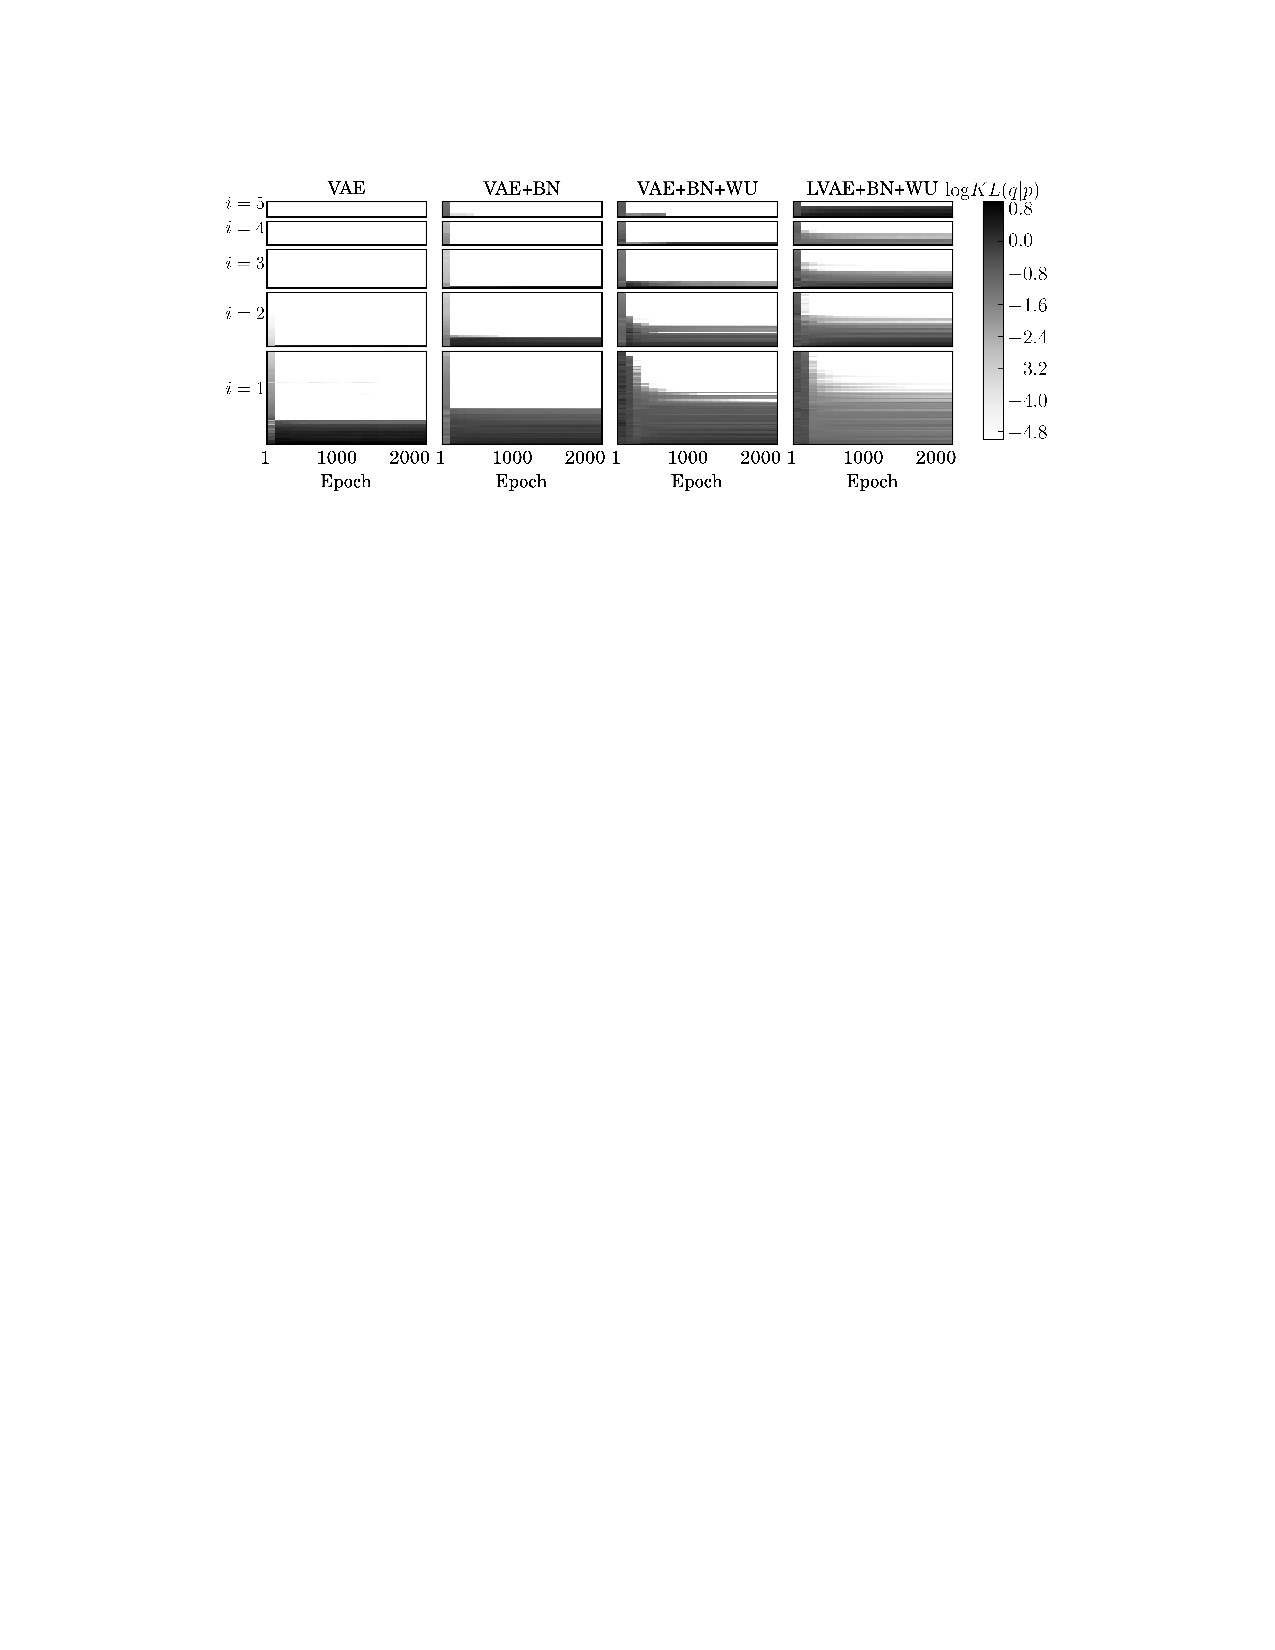
\includegraphics[scale=0.85]{figures/ladder_vae_latent_activations.pdf}
        \caption{Element-wise KL-divergences in each latent variable $q(\zb_i|\zb_{i-1})$ with $\zb_0\equiv \xb$.}
    \end{figure}
\end{frame}


\begin{frame}{Latent space representation}
    \begin{figure}[\textwidth]
        \centering
        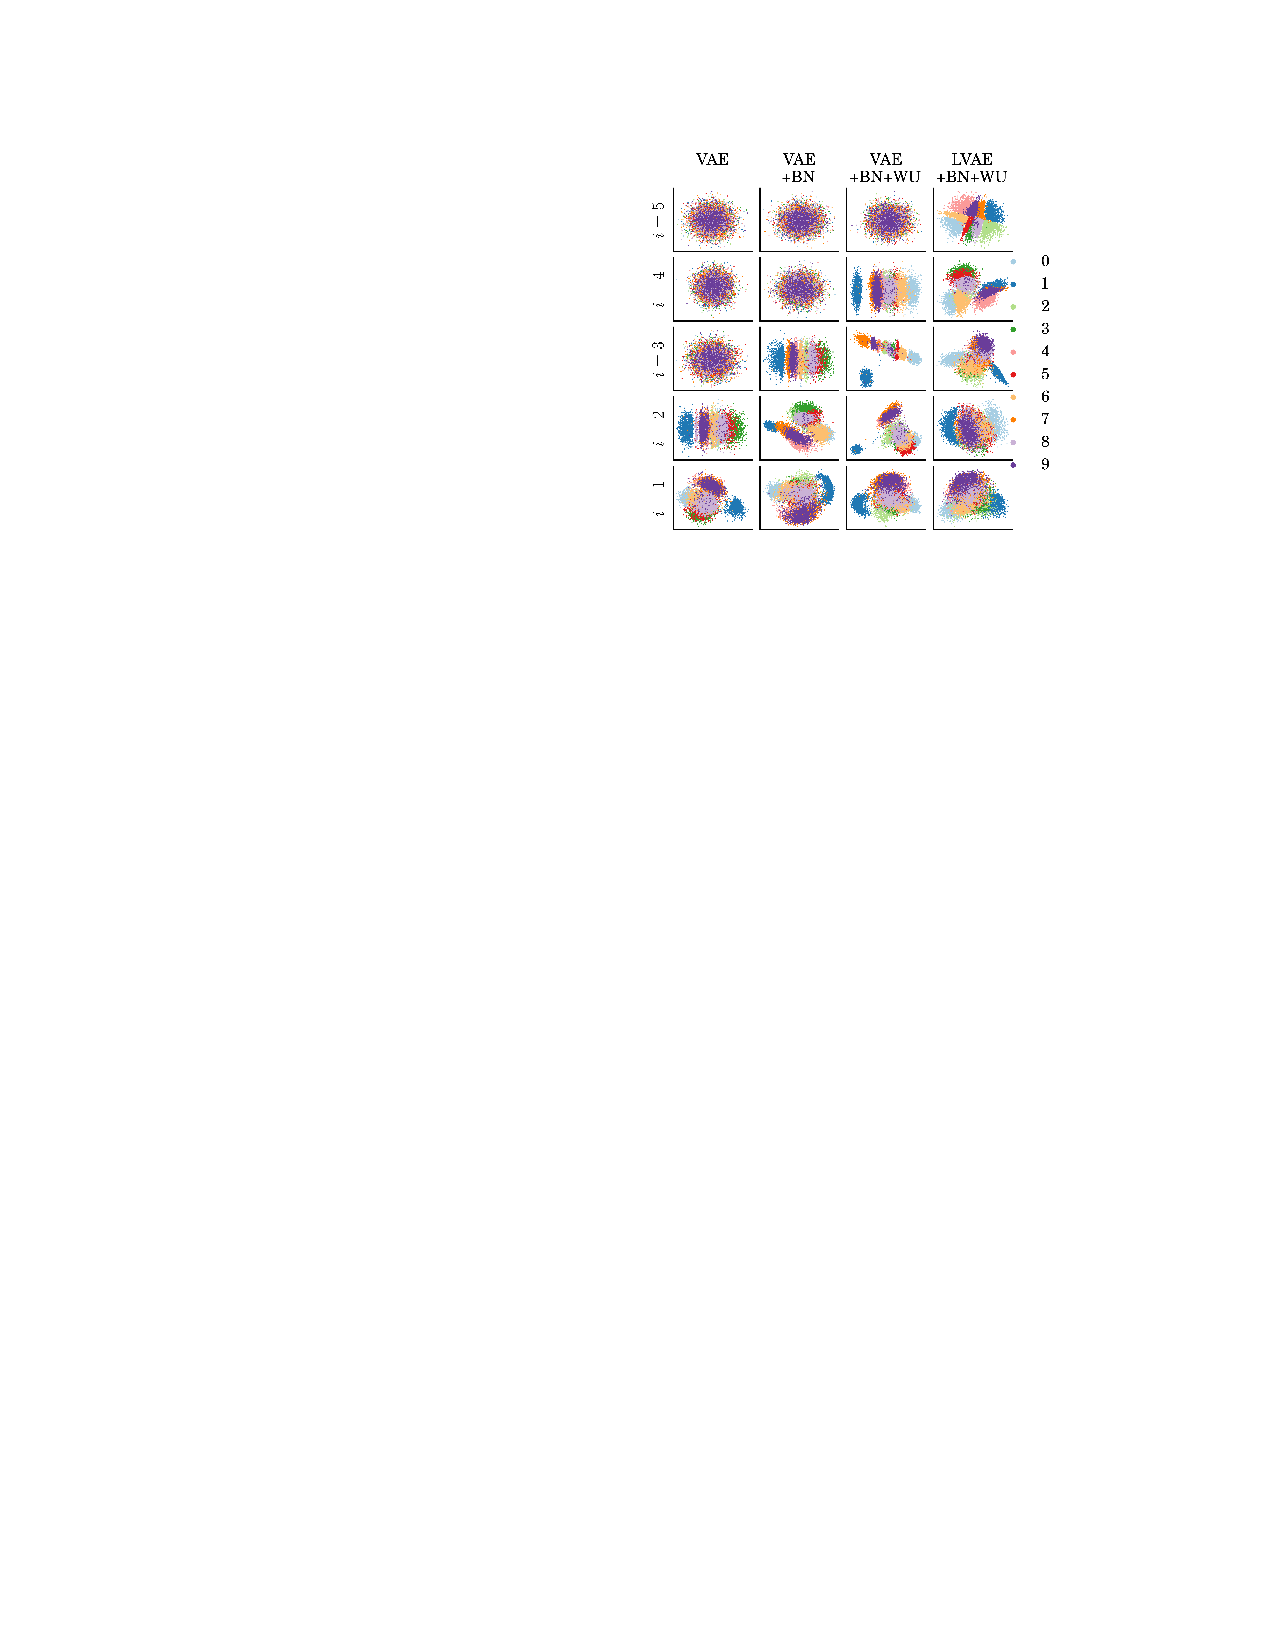
\includegraphics[scale=1]{figures/ladder_vae_pca.pdf}
        \caption{PCA of latent samples from $q(\zb_i|\zb_{i-1})$ with $\zb_0\equiv \xb$.}
    \end{figure}
\end{frame}


\begin{frame}{Recent work}
    \begin{figure}[\textwidth]
        \centering
        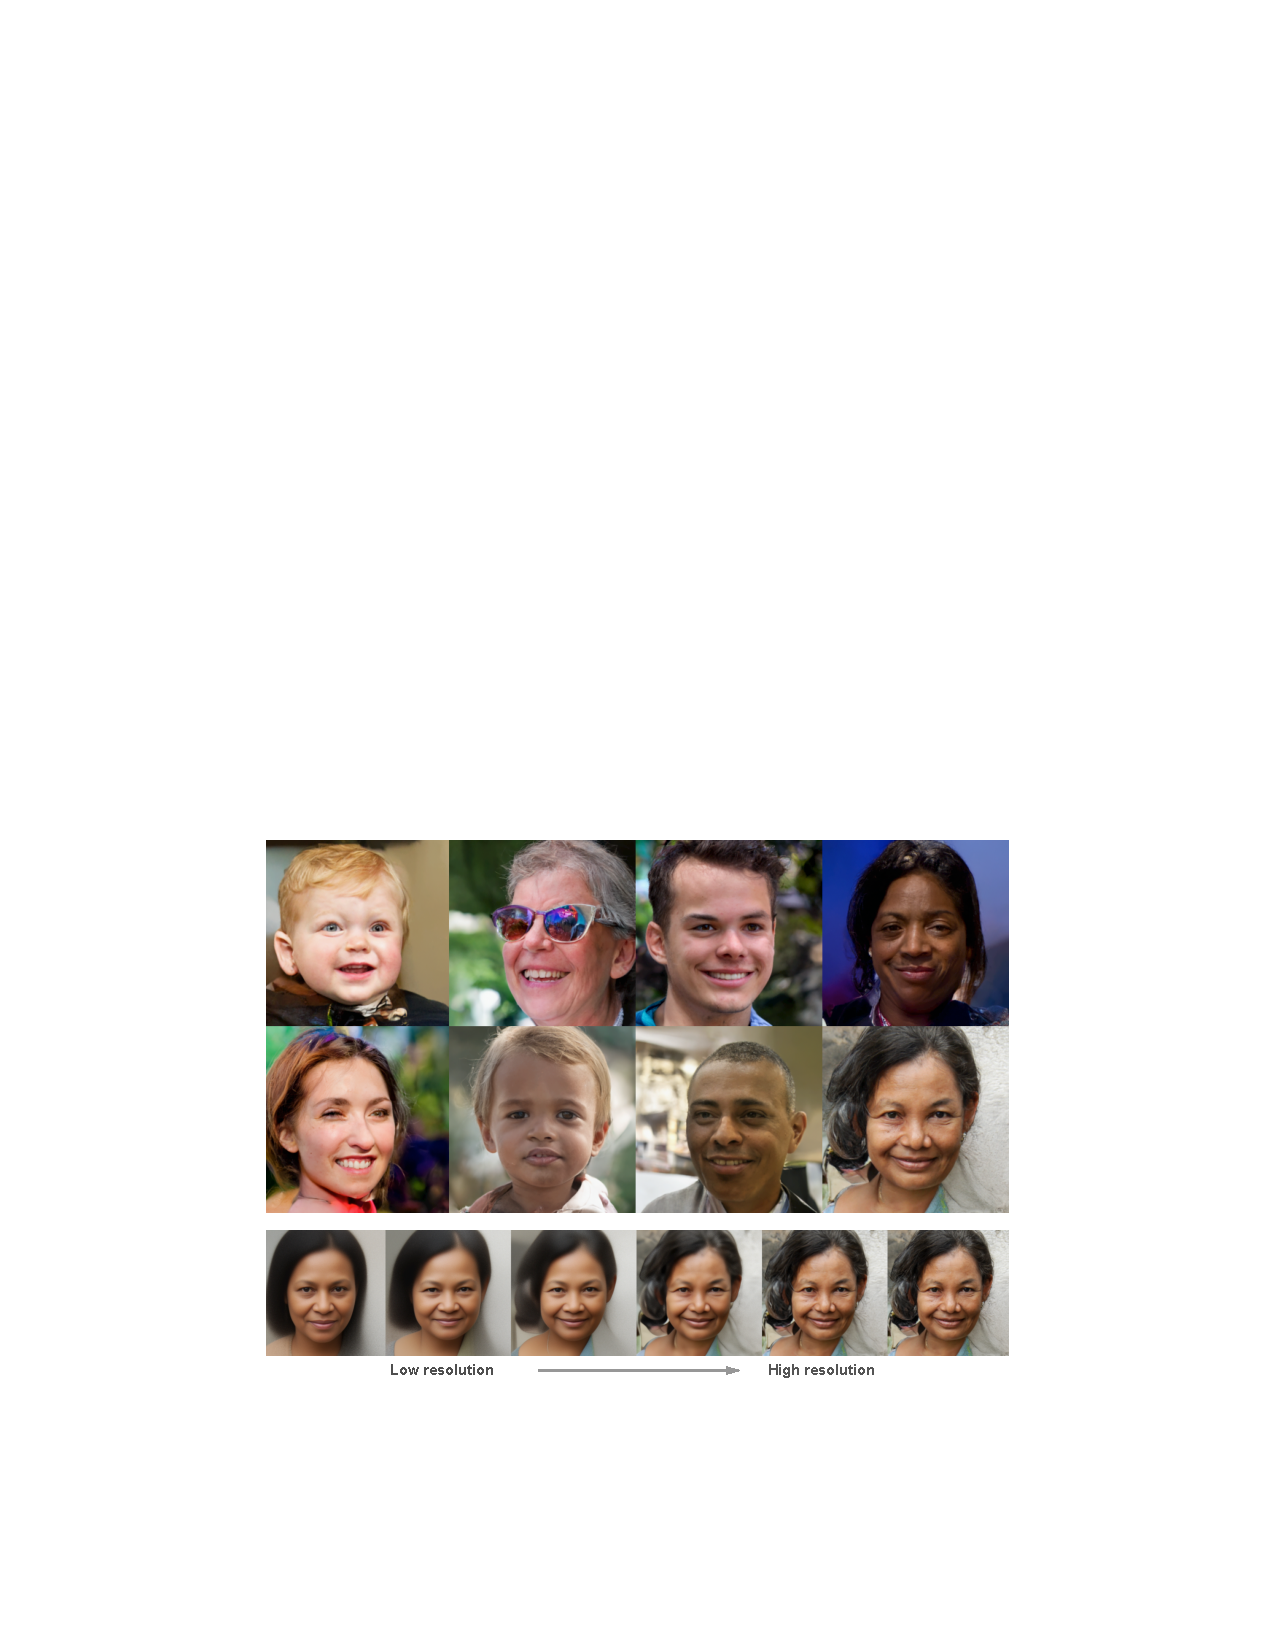
\includegraphics[scale=0.7]{figures/child_faces.pdf}
        \caption{Samples from the generative model of \cite{child_very_2021} with more than 70 latents.}
    \end{figure}
\end{frame}



% ======================================================================================================================


\section*{Overview}

\begin{frame}[allowframebreaks]
    \frametitle{Table of contents}
    \tableofcontents
\end{frame}
